\chapter{Data} \label{cha:chapter-2}

The data I am using for this project is a collection of observations of 5,960 home equity loans which is provided by \parencite{baesens2016credit}. Home equity loans are when an applicant borrows agains the value or 'equity' of their home. You can find a full description of each variable in Table (\ref{MetaData}).

\begin{table}[ht]\label{Table2}
	\centering
	\renewcommand{\arraystretch}{1.5}
	\begin{tabular}{l p{10cm}}
	\hline
	Variable & \multicolumn{1}{c}{Definition}\\ 
	\hline
	BAD & 1 = Applicant defaulted on loan or seriously delinquent; 0 = applicant pain load \\
	LOAN & Amount of requested loan \\
	MORTDUE & Amount due on exisiting mortgage \\
	VALUE & Value of property the loan is to go against \\
	REASON & The reason the applicant is applying for the loan. DebtCon = Debt condsolidation; HomeImp = Home Improvement \\
	JOB & Occupational categories \\
	YOJ & Years at present job \\
	DEROG & Number of major derogatory reports \\
	DELINQ & Number of delinquent credit lines \\
	CLAGE & Age of oldest credit line in months \\
	NINQ & Number of recent credit inquiries \\
	CLNO & Number of credit lines \\
	DEBTINC & Debt-to-income ratio \\
	\end{tabular}
	\caption{Variables used in the Data Set \label{MetaData}}
\end{table}

\section{Data Cleaning}

The data provided needed some initial cleaning. 2,596 observations were missing atleast one value with some missing several variables. The biggest culprit of this would be DEBTINC with 1,267 missing values. I decided to handle these missing values on a case by case basis applying different methods. Before I went forward with any imputing I considered any possible outliers within my numerical data, using the summary Table \ref{SUM_BFR_TBL}. You can see for the quantile ranges that there will most likely be some outliers occuring in the majority of the numerical variables. The gerneral consesus is that there is a necessity to handle outliers but a lack of definitive way to handle them \parencite{nyitrai2019effects}. For this project I chose to removed the 99th percentile for every numerical variable excluding BAD, this ended up removing 613 rows. \\

Moving onto imputing variable, for MORTDUE and VALUE I imputed their values using a simple linear regression of the other. This was going on the assumption that the mortgage due on a house had a strong relationship with the value of property. The assumption is further backed up with the correlation between the two being 0.8748 before imputing, far higher than any of the other correlations in the data. So for MORTDUE I used Equation (\ref{MORTDUE_IMPUTE}) and for VALUE I used Equation (\ref{VALUE_IMPUTE}). This was applied to any missing value where the other was present and for the remaining I took the mean of each variable from the original data before the imputations.

\begin{equation}\label{MORTDUE_IMPUTE}
\text{MORTDUE} = \beta_{0} + \beta_{1}\text{VALUE}
\end{equation}

\begin{table}[ht]\label{MORTDUE_IMPUTE_COEFS}
	\centering
	\begin{tabular}{lr}
	\hline
	$\beta_{0}$ & -2145.6497 \\
	$\beta_{1}$ & 0.7177 \\
	\hline
	\end{tabular}
\end{table}

\begin{equation}\label{VALUE_IMPUTE}
\text{VALUE} = \beta_{0} + \beta_{1}\text{MORTDUE}
\end{equation}

\begin{table}[ht]\label{VALUE_IMPUTE_COEFS}
	\centering
	\begin{tabular}{lr}
	\hline
	$\beta_{0}$ & 21340.4803 \\
	$\beta_{1}$ & 1.1253 \\
	\hline
	\end{tabular}
\end{table}

For the remaining numerical variables excluding DEBTINC I chose to take the median of the values as there were only a small amount missing from each but still a significant amount $( > 4\% )$ missing. There is an argument that because DEBTINC is missing 1,081 (20.2 \%) that some other method from using the median value should be used. After some further analysis the decsion to drop the variable was made, imputing did not appear to be an option as of the 915 bad applicants,  634 (69.3\%) of them were missing DEBTINC compared to 4432 and 447 (10.1\%) for good applicants. Dropping every row with DEBTINC did not appear to be practical either as it would result in the loss of almost 70\% of the bad applicants and their data whilst also taking the bad rate down to 6\%. Dropping DEBTINC would be the lower loss of information against the alternative of dropping missing rows (5,347 values lost versus 12,972). \\

Last was the two categorical variables REASON ( DebtCon,  HomeImp ) and JOB ( Other,  Office,  Sales,  Mgr,  ProfExe,  Self ). REASON's categories were specified in the data dictionary but JOB's categories were not. The decision was made to use listwise deletion on these as they were the only variables remaining with missing data. This resulted in the removal of 377 rows. \\

With these two completed I had no more missing values and no other noticeable issues which needed to be corrected before I could further look into the variables. A summary of actions taken on missing values can be found in Table (\ref{DataCleanSummary}). \\

\begin{table}[ht]
	\centering
	\renewcommand{\arraystretch}{1.25}
	\begin{tabular}{l r p{9cm}}
	\hline
	Variable & \multicolumn{1}{c}{No. Missing} & \multicolumn{1}{c}{Solution}\\ 
	\hline
	BAD & 0 & N/A\\
	LOAN & 0 & N/A \\
	MORTDUE & 477 & Imputed from a linear regression (\ref{MORTDUE_IMPUTE}). Mean taken when VALUE was unavailable \\
	VALUE & 86 & Imputed from a linear regression (\ref{VALUE_IMPUTE}). Mean taken when MORTDUE was unavailable \\
	REASON & 222 & Listwise deletion \\
	JOB & 258 & Listwise deletion \\
	YOJ & 486 & Median taken\\
	DEROG & 655 & Median taken \\
	DELINQ & 548 & Median taken\\
	CLAGE & 303 & Median taken \\
	NINQ & 476 & Median taken\\
	CLNO & 222 & Median taken \\
	DEBTINC & 1081 & Variable dropped as too much information missing\\
	\end{tabular}
	\caption{Missing Variables Breakdown \label{DataCleanSummary}}
\end{table}

\section{Variables}\label{sec:variables}

With data cleaned the remaining observations was 4970 of 12 independ variables with no missing values. A summary of the numerical values can be found in Table (\ref{SUM_AFT_TBL}). There you can see the remaining data has a bad rate of 18\% which equates to 876 defaulted applicants.

\subsection*{LOAN}

LOAN,  the amount requested for the home equity loan by the applicant can be seen in Figure (\ref{loan_dist}). The initial assumption was that higher loan values would have a higher bad rate due to the larger amount to pay back,  increasing the length and difficulty for the applicant to pay back the loan. Looking at the figure this does not appear to be the case,  although small,  larger loans tend to be payed off more often. The reasons for this are unclear,  a couple suggested could be that since we do not know exactly how this data was gathered the case could be that for larger loans the bank/company offering these loans had higher cutoffs on their applicant scoring to prevent higher risks in higher potential loss causing a shift down in the bad rate. Another could be the arguement that larger requested loans are coming from owners of higher valued properties,  which could be the case when looking at the correlation Table (\ref{CORR_TBL}). A higher property value indicates a better economic status and less likely to default on a loan. It would be reasonable to expect this variable to have a significant effect on the credit score.

\begin{figure}[H]
	\centering
	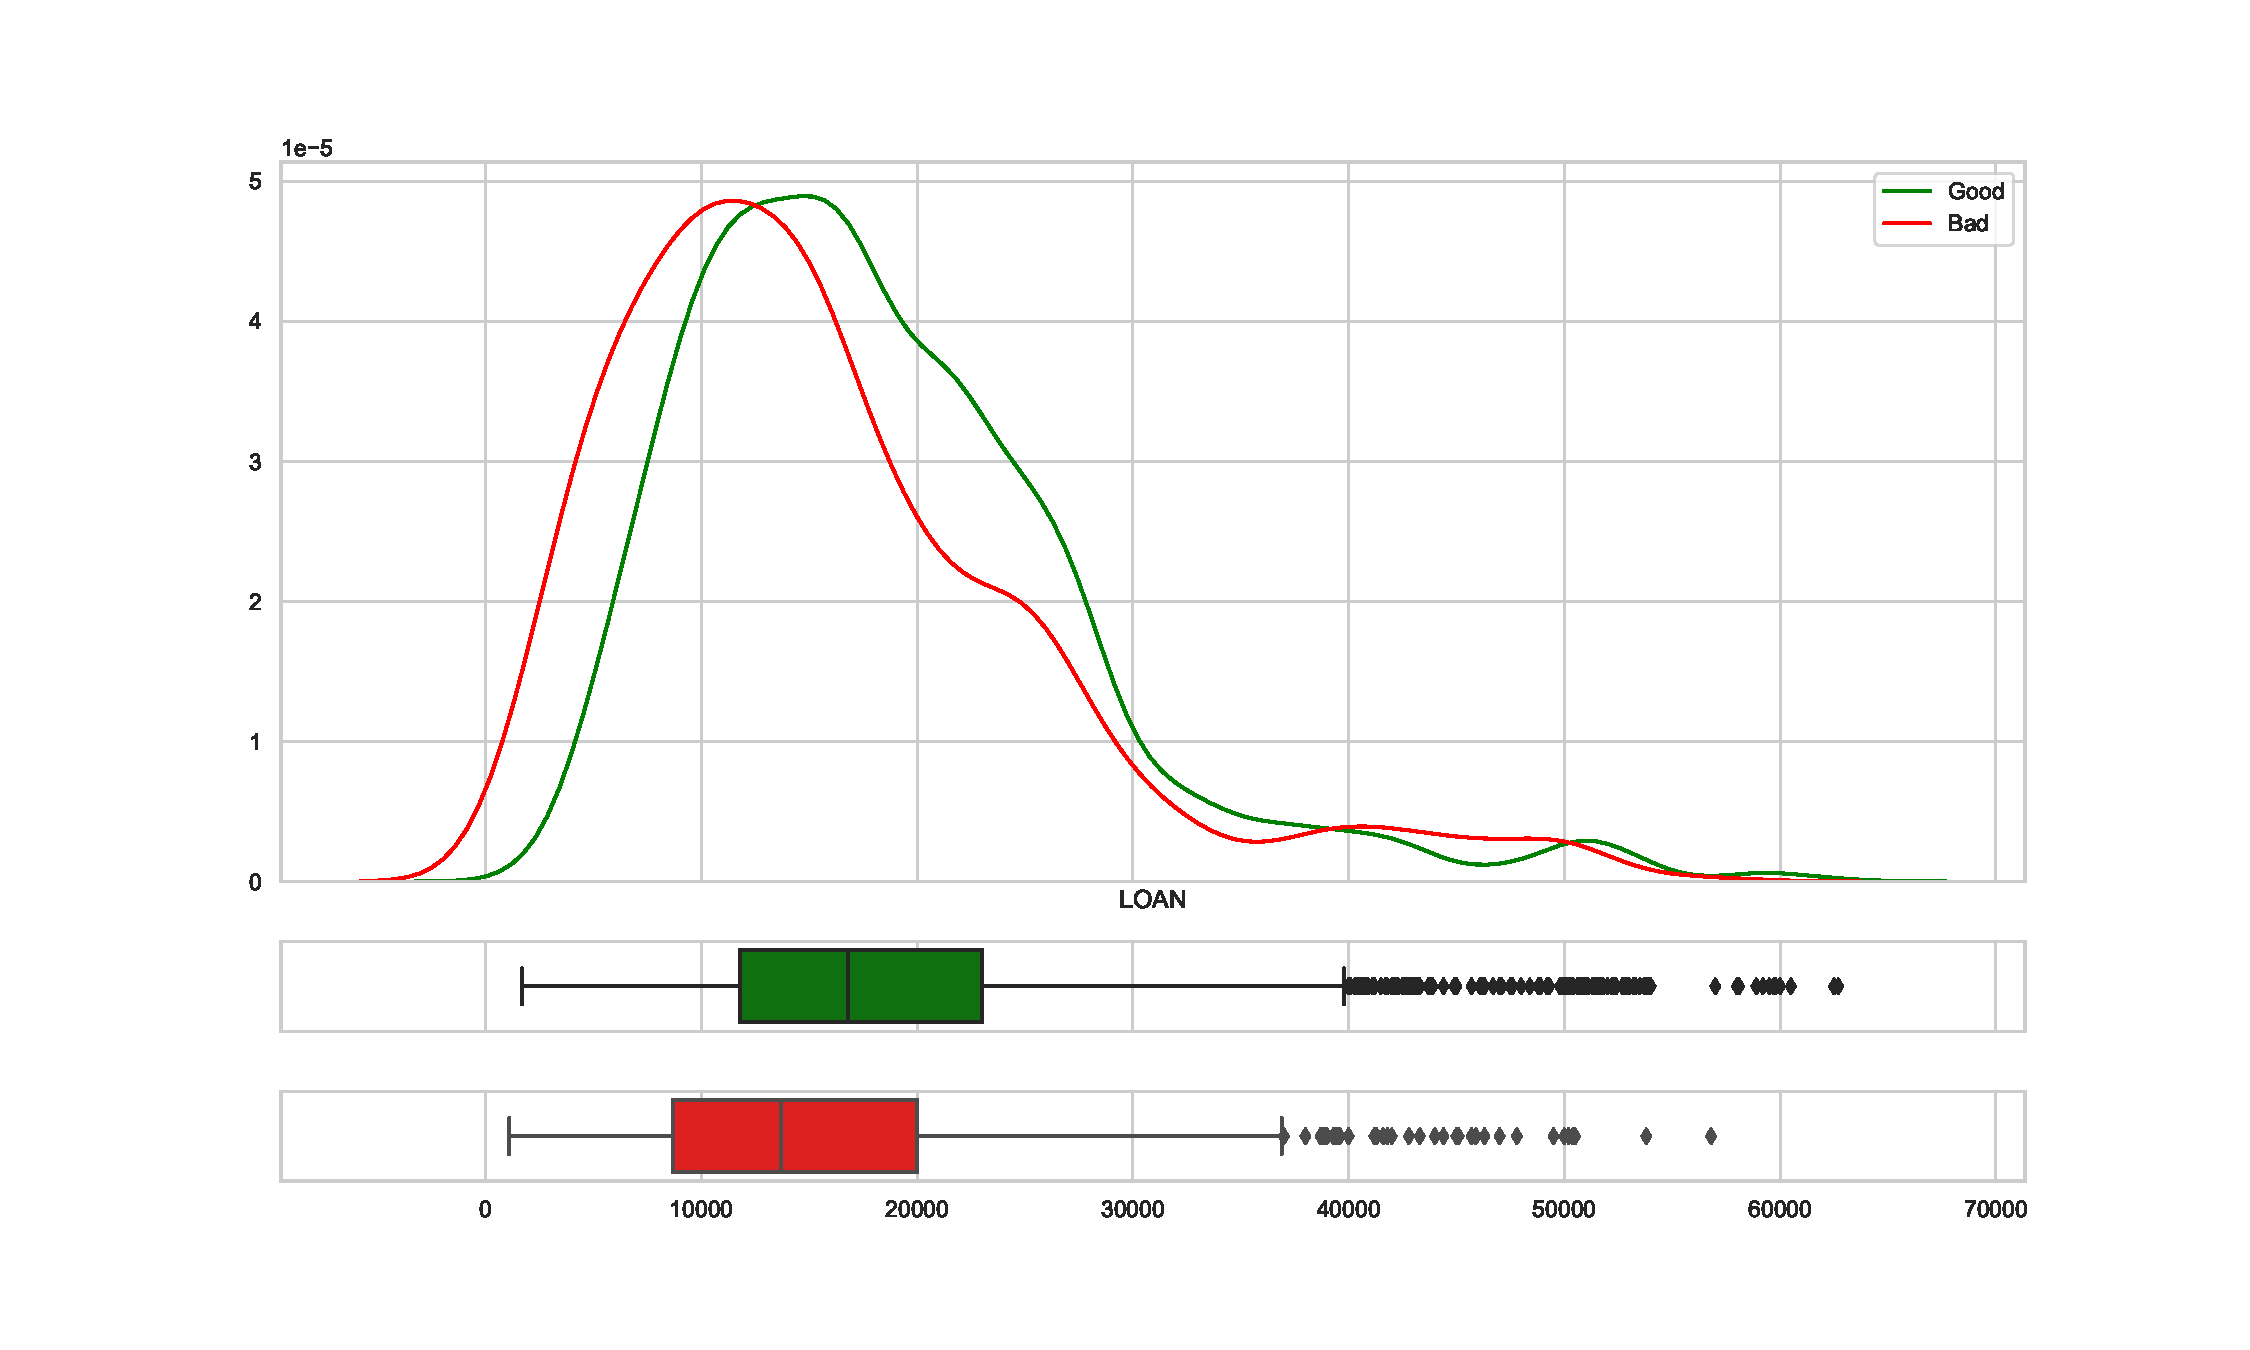
\includegraphics[scale=0.40]{figs/loan_dist.pdf}
	\caption{Distribution of LOAN by BAD. \label{loan_dist}}
\end{figure}

\subsection*{MORTDUE}

MORTDUE,  the outstanding balance on the applicants existing mortgage. Assumption here would be similar to LOAN,  a higher outstanding balance on their mortgage mean a large amount of debt and an increased risk of defaulting due to the larger payments. Looking at Figure (\ref{mortdue_dist}) you can see it does not follow this assumption,  again a small but clear difference in the distribution shows that applicants with a higher outstanding balance on their mortgage are less likely to default. Whatever the reason behind this is would most likely be the same as the reason behind LOAN.

\subsection*{VALUE}

VALUE,  the property of the applicants and the equity the loan is being put against. The same initial assumption being made with MORTDUE is also here,  a value of an applicants property is an indication of their economic status. An owner of a higher valued property should be able to payback a larger loan and less likely to default on smaller ones. From Figure (\ref{value_dist}) there is a small visible effect of loan on their probability of defaulting.

\begin{figure}[H]
	\centering
	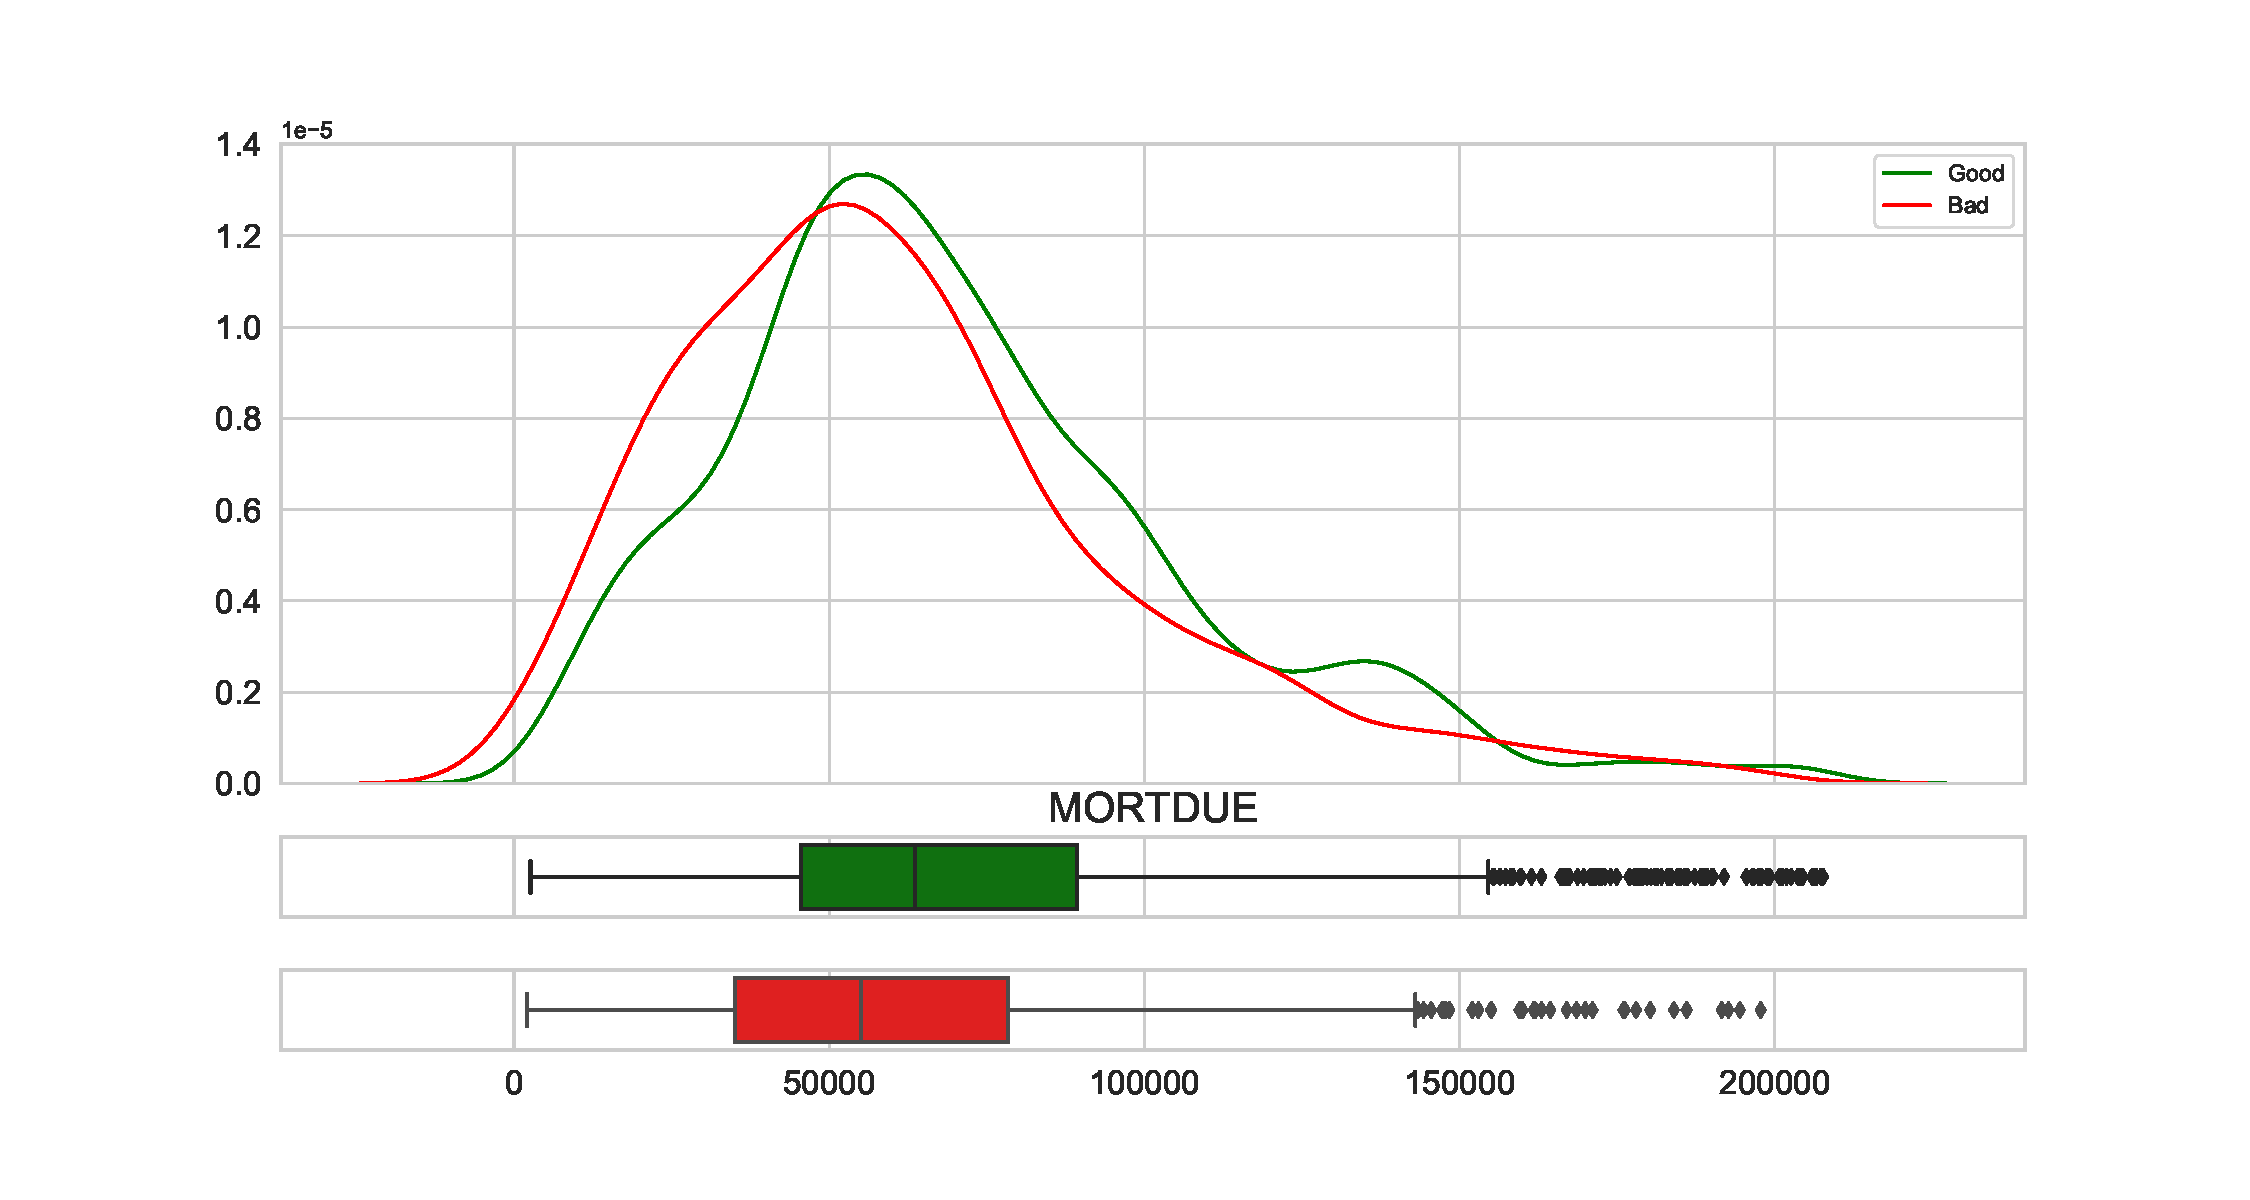
\includegraphics[scale=0.40]{figs/mortdue_dist.pdf}
	\caption{Distribution of MORTDUE by BAD. \label{mortdue_dist}}
\end{figure}

\begin{figure}[H]
	\centering
	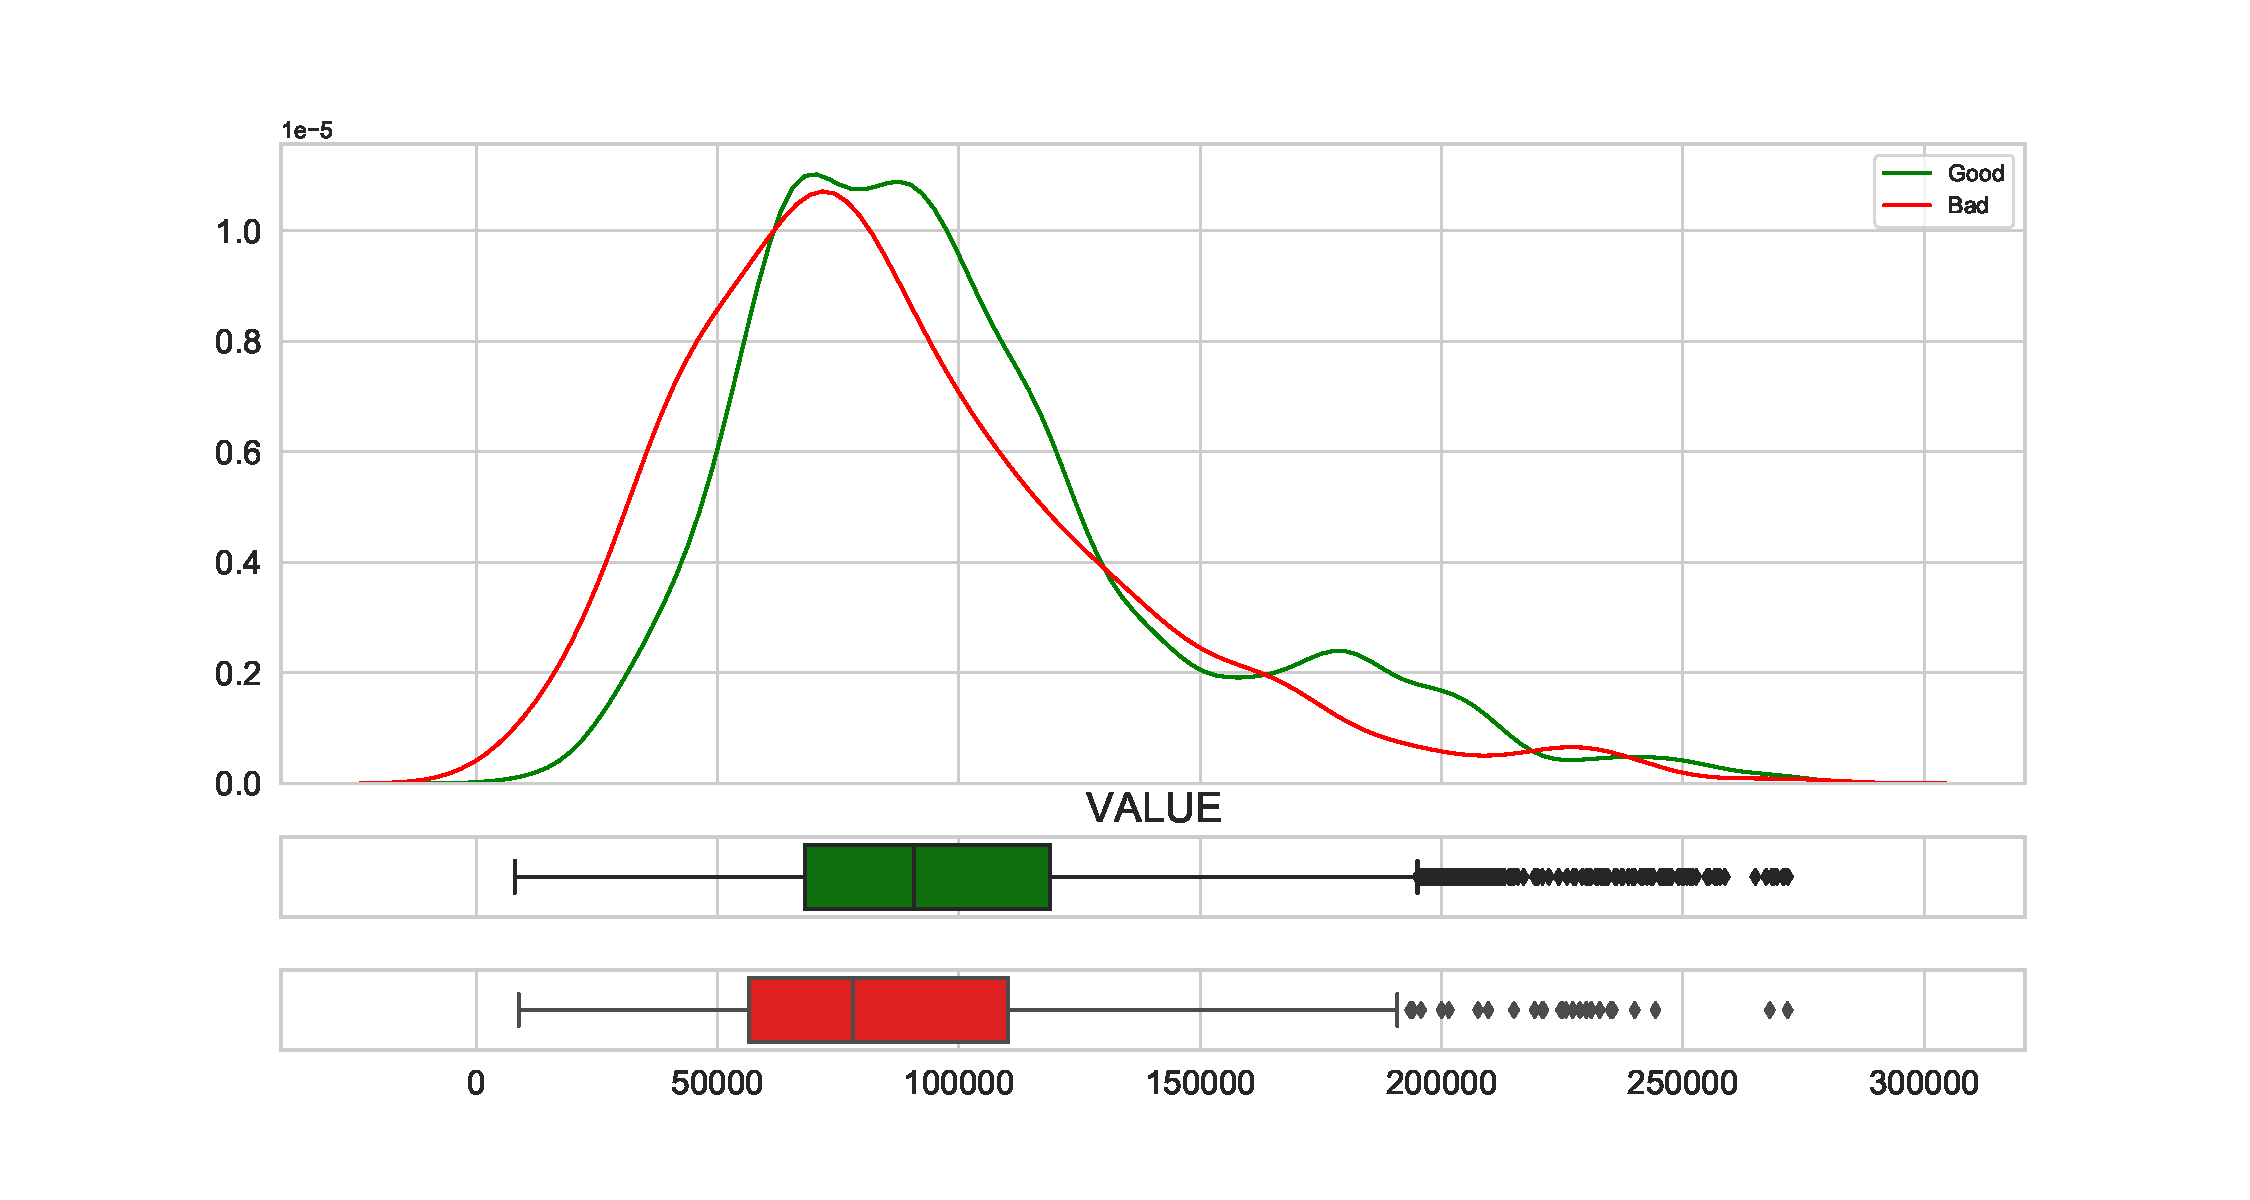
\includegraphics[scale=0.40]{figs/value_dist.pdf}
	\caption{Distribution of VALUE by BAD. \label{value_dist}}
\end{figure}

\subsection*{REASON}

REASON,  the reason for the applicant's request. There are only two categories as seen in \ref{reason_cat},  DebtCon,  the loan would be used for a debt consolidation. HomeImp,  the loan is being used for a home improvement. A breakdown of their splits between good and bad can be found in Table (\ref{reason_count_tbl}). The two categories continue to have similar splits when they do not default but when they do default,  HomeImp's split increases by 7\%. Looking at this further in Figure (\ref{reason_cat}) the bad rate for DebtCon is 16.24\% and HomeImp 20.75\%. Although there does appear to be a difference,  it is small and compared to other variables in the group I would expect this to be on the lower end of signifiance.

\begin{table}[H]
	\centering
	\renewcommand{\arraystretch}{2}
	\begin{tabular}{lrrr}
		\toprule
		Category & \% of Total (N = 4970) & \% of Good (N = 4094) & \% of Bad (N = 876) \\
		\midrule
		DebtCon &  69.3\% (3442) & 70.4\% (2883) & 63.8\% (559)  \\
		HomeImp & 30.7\% (1528) & 29.6\% (1211) &  36.2\% (317)  \\
		\bottomrule
	\end{tabular}
	\caption{REASON breakdown \label{reason_count_tbl}}
\end{table}

\begin{figure}[H]
	\centering
	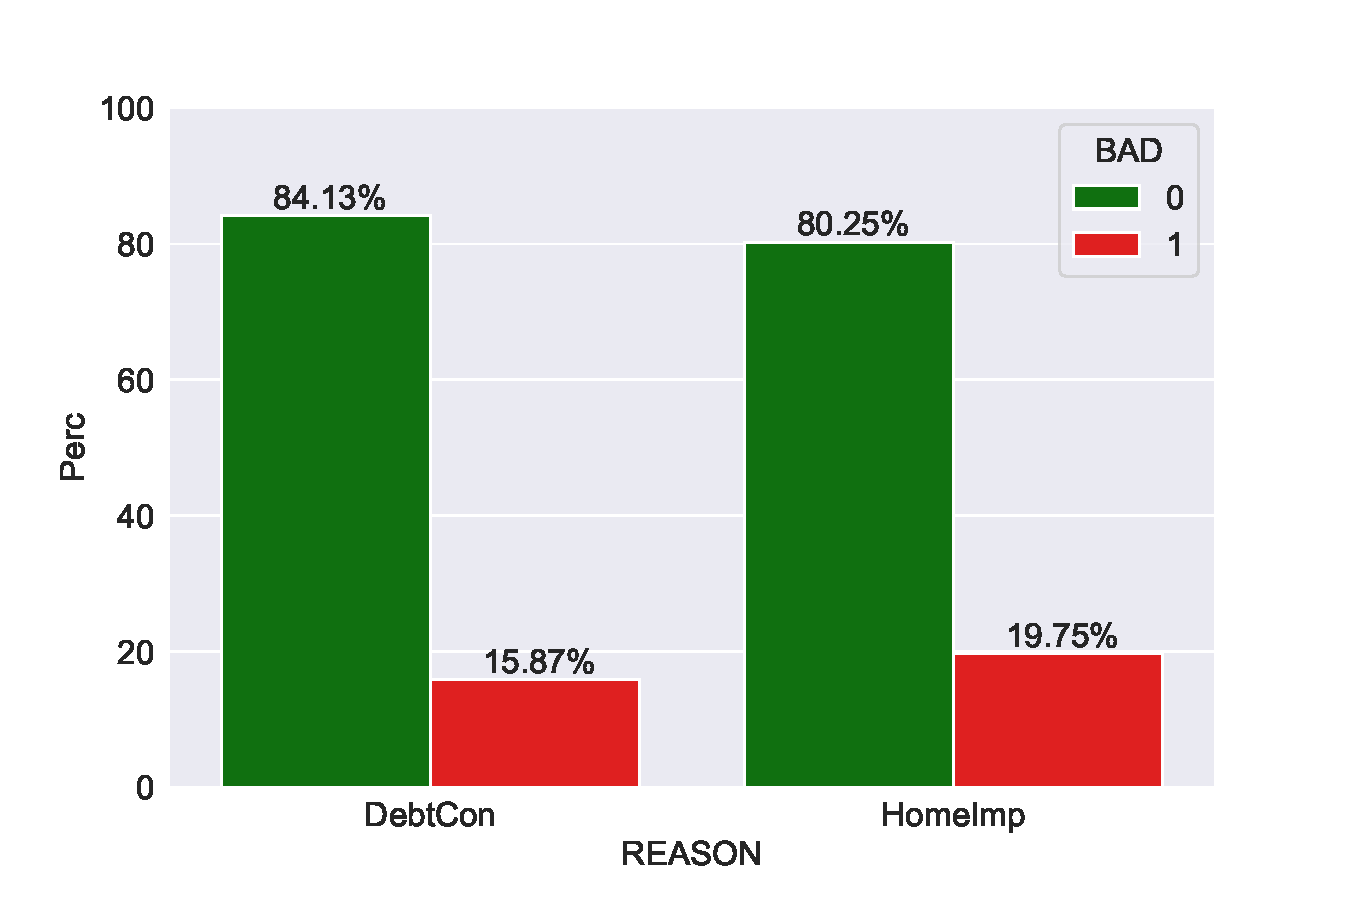
\includegraphics[scale=0.40]{figs/reason_cat.pdf}
	\caption{Category plot of REASON by BAD. \label{reason_cat}}
\end{figure}

\subsection*{JOB}

JOB, categorical job occupation. Categories can be seen in \ref{job_cat}. Occupation could be used as an indicator for the applicants economic status e.g. a ProfExe, proffesional executive is more likely to have a higher income than office staff or someone who is self employed. It could also be used to see how volatile their employement status is, someone who is self employed can be seen as a possible risk due to their income being potentially unstable. Although we do not have a way of looking at their job security,  we do have YOJ,  years at present job, as an indicator of Job security. Comparing Figure (\ref{job_yoj_cat}) and Figure (\ref{job_cat}), Sales, the job with the lowest average YOJ has the highest bad rate at 31.52\% followed by Self at 24.14\%. 

\begin{table}[H]
	\centering
	\renewcommand{\arraystretch}{2}
	\begin{tabular}{lrrr}
		\toprule
		Category & \% of Total (N = 4970) & \% of Good (N = 4094) & \% of Bad (N = 876) \\
		\midrule
		Other & 42.5\% (2110) & 40.7\% (1666) &  50.7\% (444)  \\
		ProfExe & 22.5\% (1119) & 23.9\% (977) &  16.2\% (142)  \\
		Office & 17.0\% (844) & 18.2\% (746) &  11.2\% (98)  \\
		Mgr &  13.3\% (660) & 13.0\% (532) & 14.6\% (128)  \\
		Self & 2.9\% (145) & 2.7\% (110) &  4.0\% (35)  \\
		Sales & 1.9\% (92) & 1.5\% (63) &  3.3\% (29)  \\
		\bottomrule
	\end{tabular}
	\caption{JOB breakdown \label{job_count_tbl}}
\end{table}

\begin{figure}[H]
	\centering
	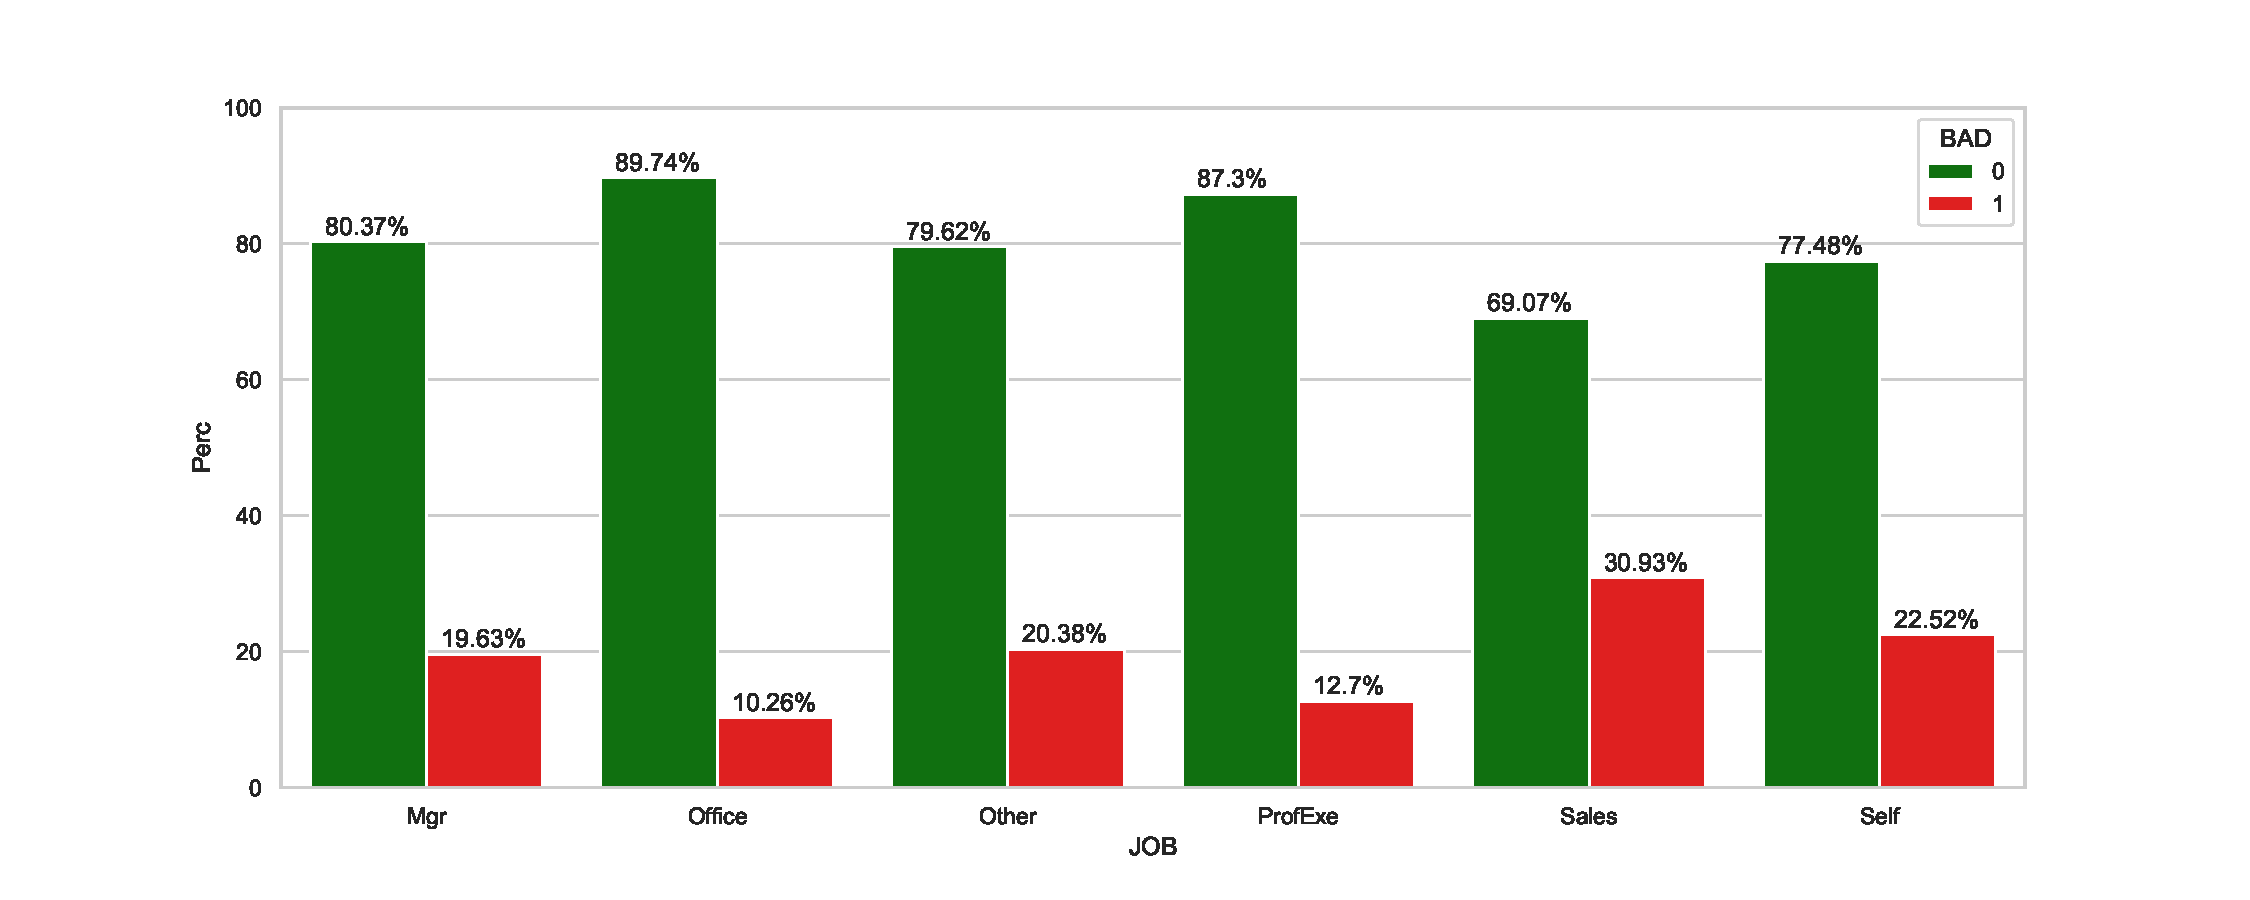
\includegraphics[scale=0.40]{figs/job_cat.pdf}
	\caption{Category plot of JOB by BAD. \label{job_cat}}
\end{figure}

\begin{figure}[H]
	\centering
	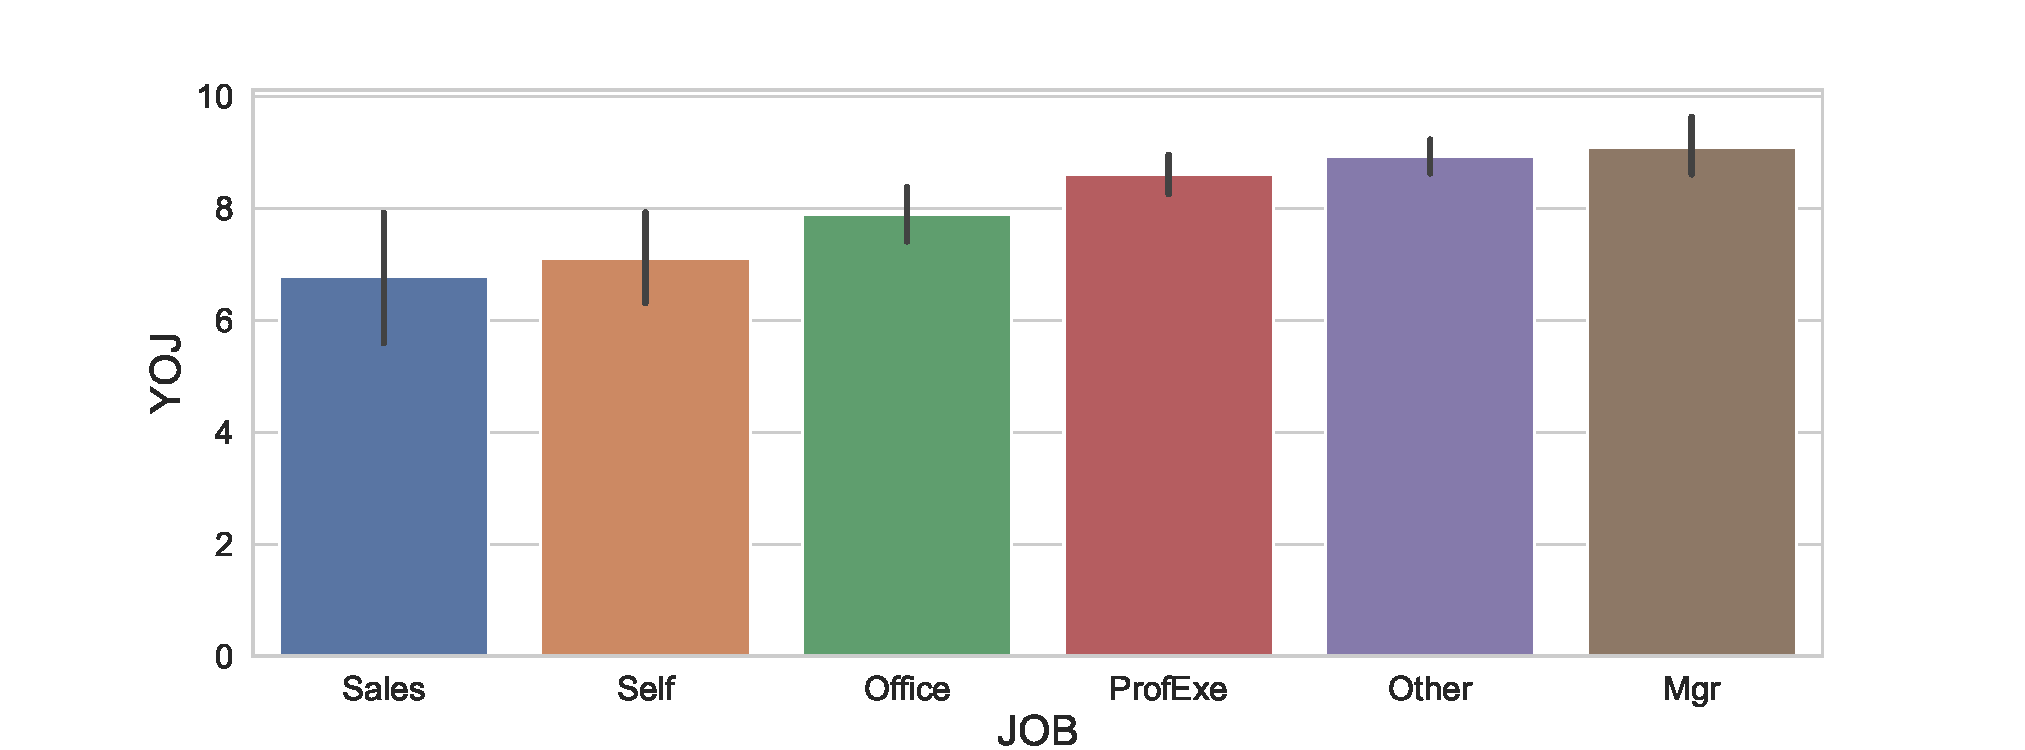
\includegraphics[scale=0.40]{figs/job_yoj_cat.pdf}
	\caption{Category plot of JOB by mean of YOJ. \label{job_yoj_cat}}
\end{figure}

\subsection*{YOJ}

YOJ, number of years the applicant has been at present job. Can be an indicator of job security,  an applicant losing their job can be a high risk of defaulting on their loan. Figure (\ref{yoj_dist} shows that the majority of applicants are between 3 to 14 years at their current job with the mean for bads and goods being relatively the same. The difference between them starts to become noticable at higher values where an applicant who has been at their present job for more than 20 years starts to become less likely to default.

\begin{figure}[H]
	\centering
	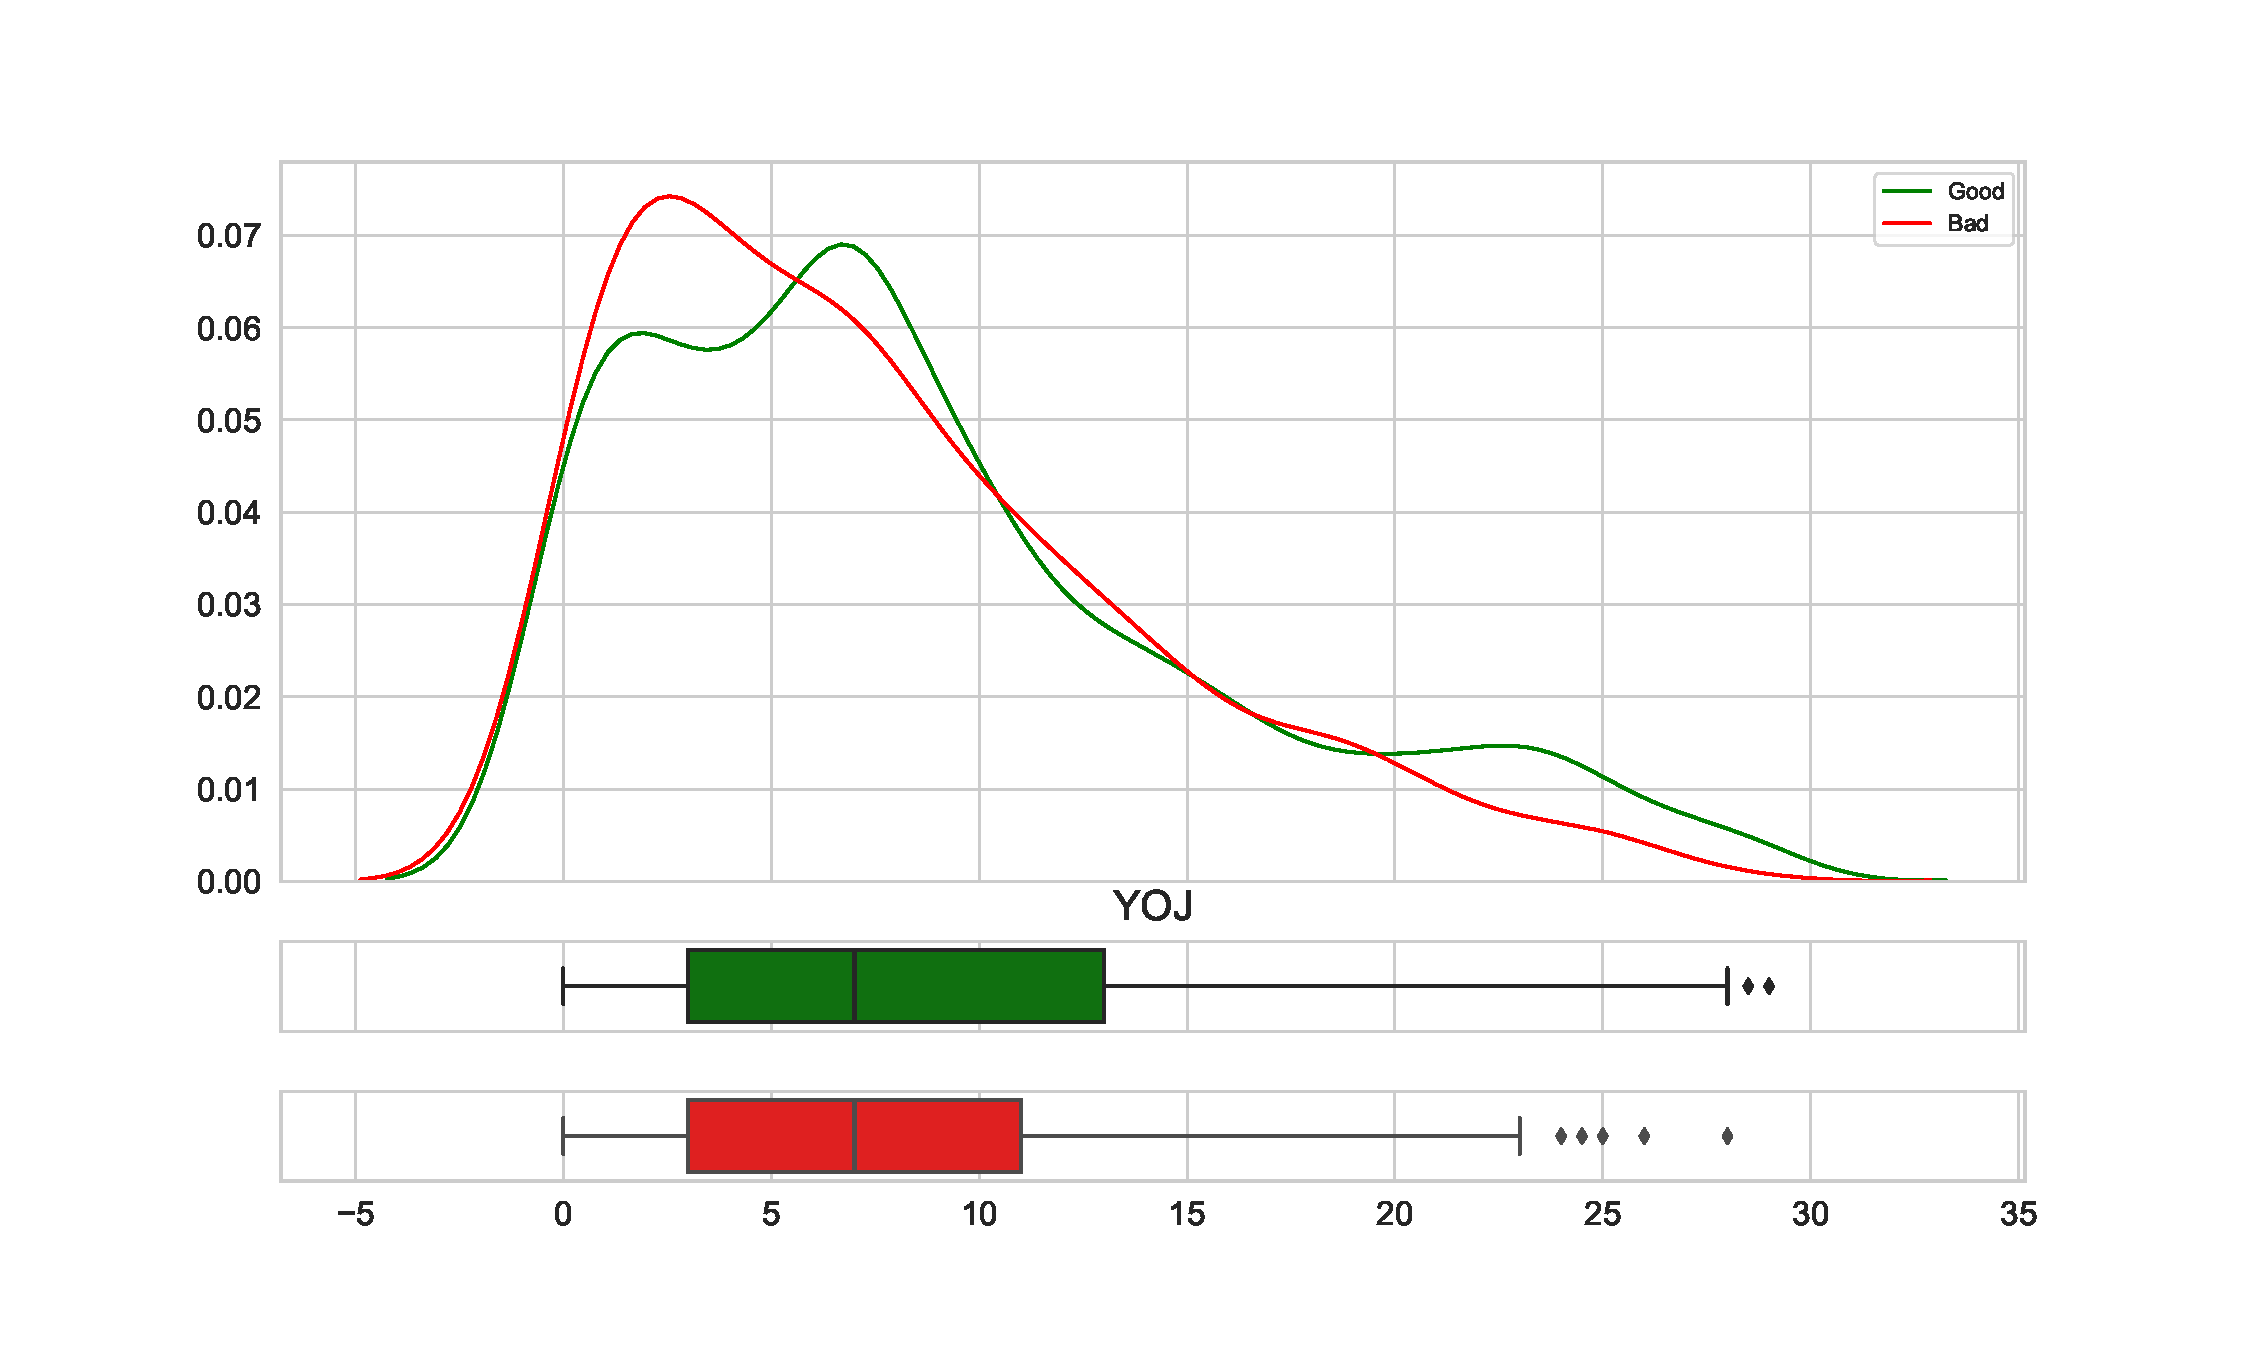
\includegraphics[scale=0.40]{figs/yoj_dist.pdf}
	\caption{Distribution of YOJ by BAD. \label{yoj_dist}}
\end{figure}

\subsection*{DEROG}

DEROG,  number of dergoatory marks on aginast the applicant. A derogatory mark can have a large impact on your chances of being accepted for a loan. In this dataset,  only 12.3\% of applicants have 1 or more dergoatory mark. An applicant can recieve a derogatory mark for various reasons such as,  missing payments,  bankruptcy,  repossession,  etc. The severity of the reason for the derogatory mark is often used in credit scoring but for this dataset we only have the numbers of marks against the applicant. Figure (\ref{derog_cat}) shows the impact having a derogatory mark can have on your chance of defaulting with 0 having a bad rate of 15.04\% and 3 having a bad rate of 65.12\%.

\begin{figure}[H]
	\centering
	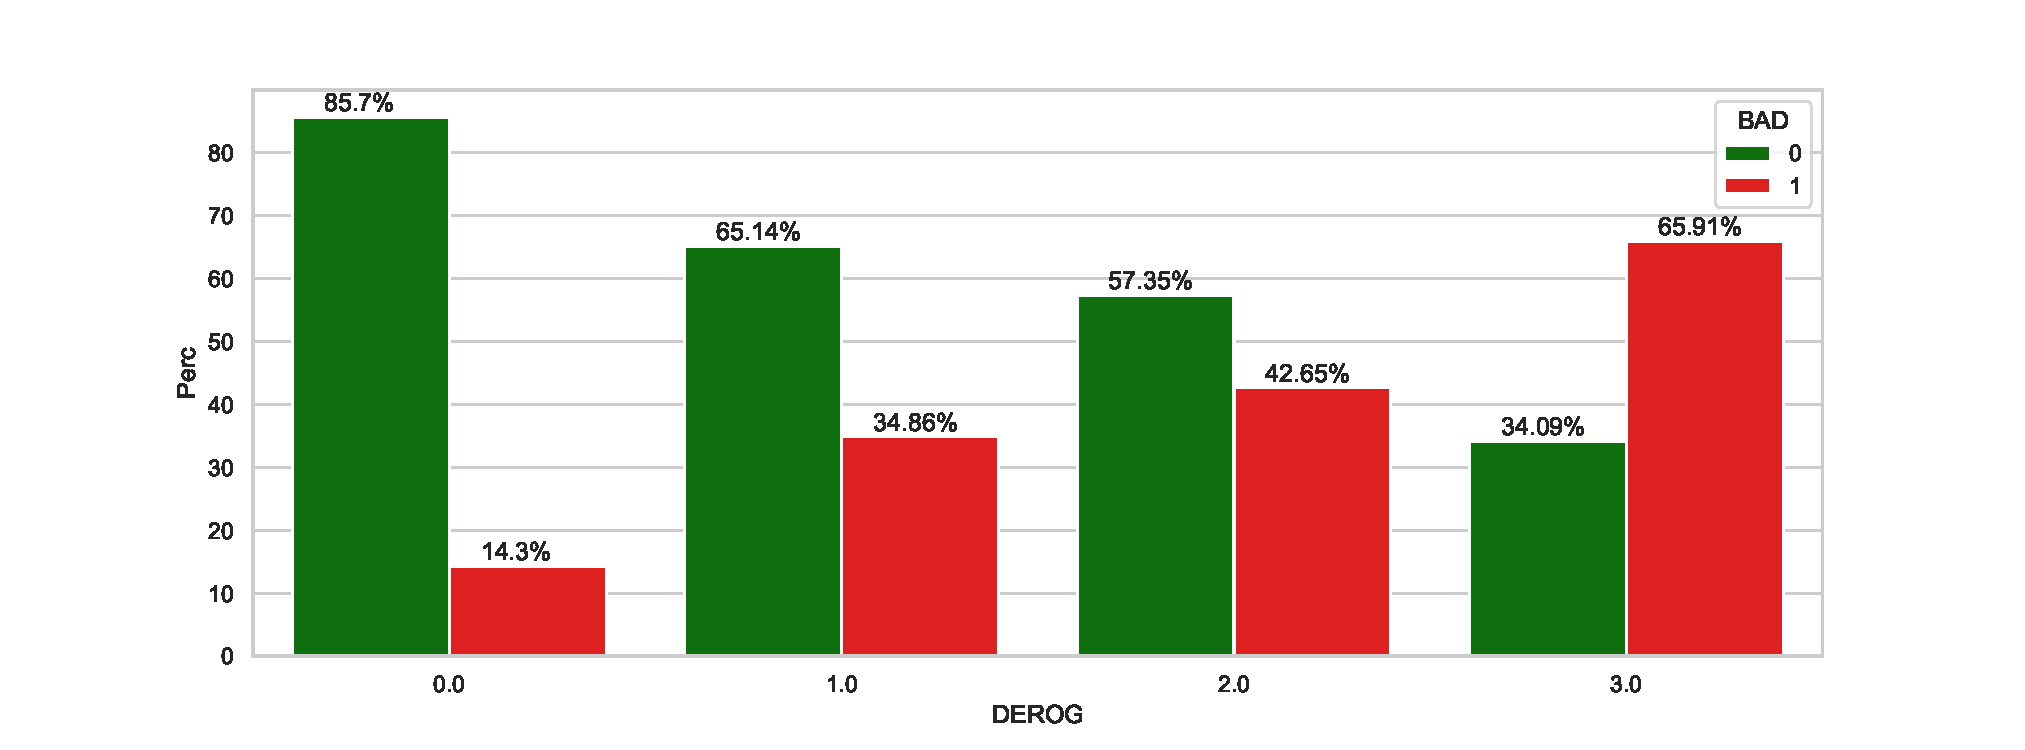
\includegraphics[scale=0.40]{figs/derog_cat.pdf}
	\caption{Category plot of DEROG by BAD. \label{derog_cat}}
\end{figure}

\subsection*{DELINQ}

DELINQ,  Number of delinquent credit lines. Delinquency is used to describe when a borrower has missed a payment,  the borrower is referred to as delinquent. Delinquency preceeds defaulting,  once a borrower has been deqlinquent for a time it comes apparent that the borrower is unable to pay back the loan. The data we are provided is the number of deqlinquent credit lines,  which is the number of credit lines the borrower has missed payments on. 

\begin{figure}[H]
	\centering
	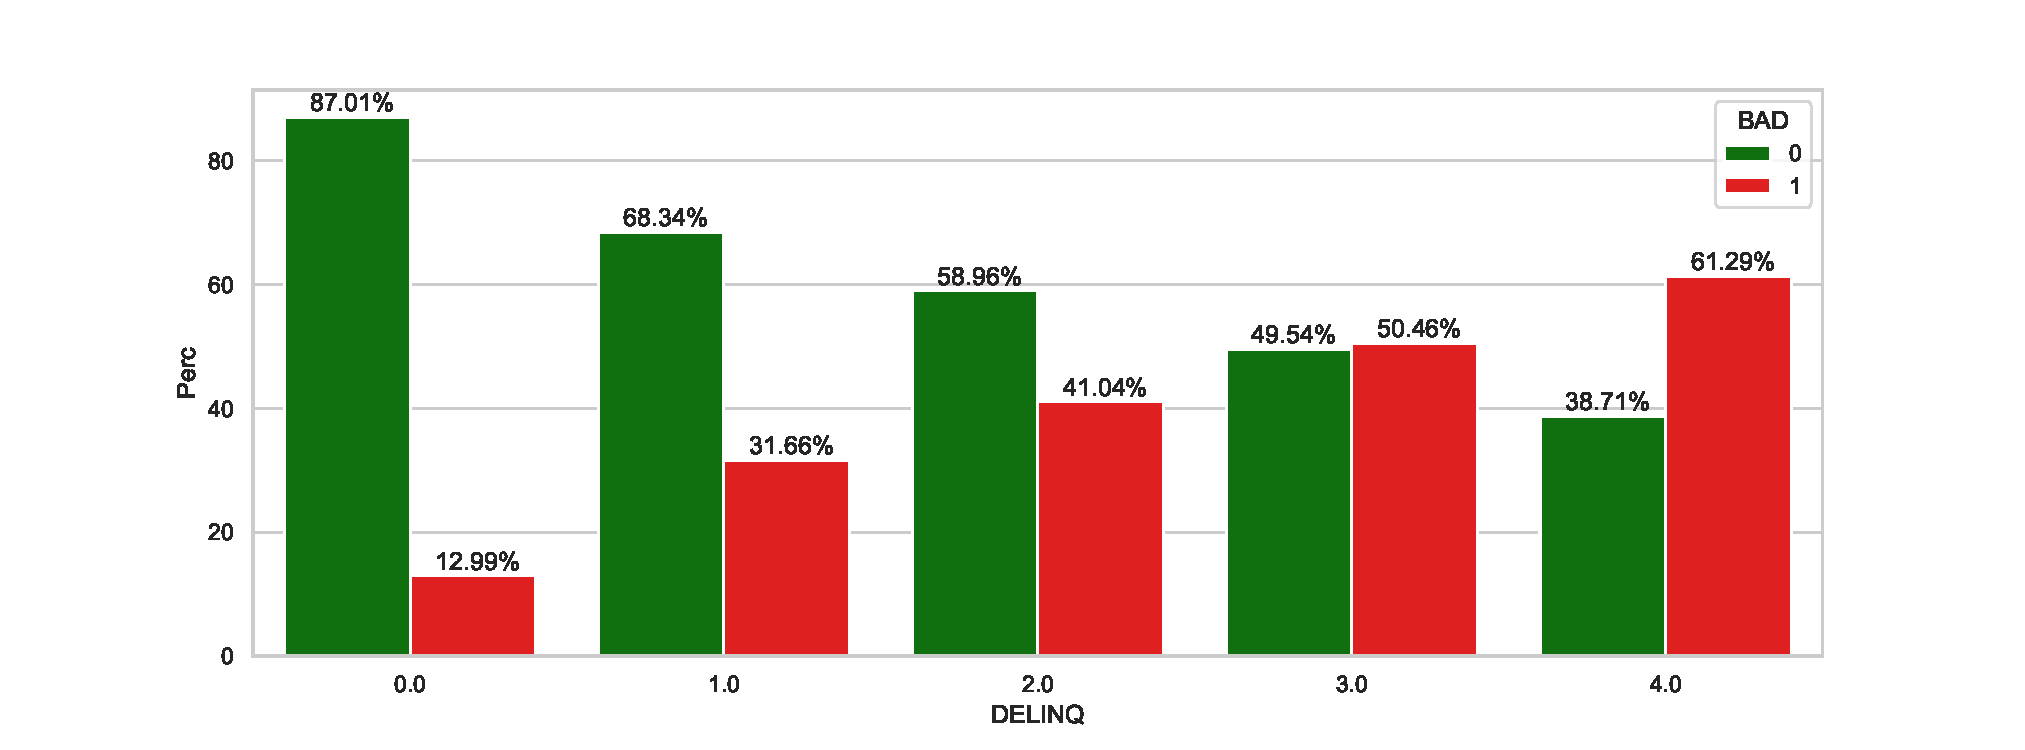
\includegraphics[scale=0.40]{figs/delinq_cat.pdf}
	\caption{Category plot of DELINQ by BAD. \label{delinq_cat}}
\end{figure}

\subsection*{CLAGE}

CLAGE,  Age of oldest credit line in months. Assumption here is the longer an applicant has held credit lines the more experienced they are in repaying payments. A applicant who has experience in credit repayments for 20 years is going to have a better time in avoiding delinqency and defaulting that someone who is new to credit. Figure (\ref{clage_dist}) reinforces this assumption,  there is a clear difference in the distributions of goods and bads. Applicants between 100 and 150 months on thier oldest credit line have a bad rate of 21.8\% and applicants between 200 and 300 have a bad rate of 9.5\%. Expecting this value to have a strong signifance for the credit score.

\begin{figure}[H]
	\centering
	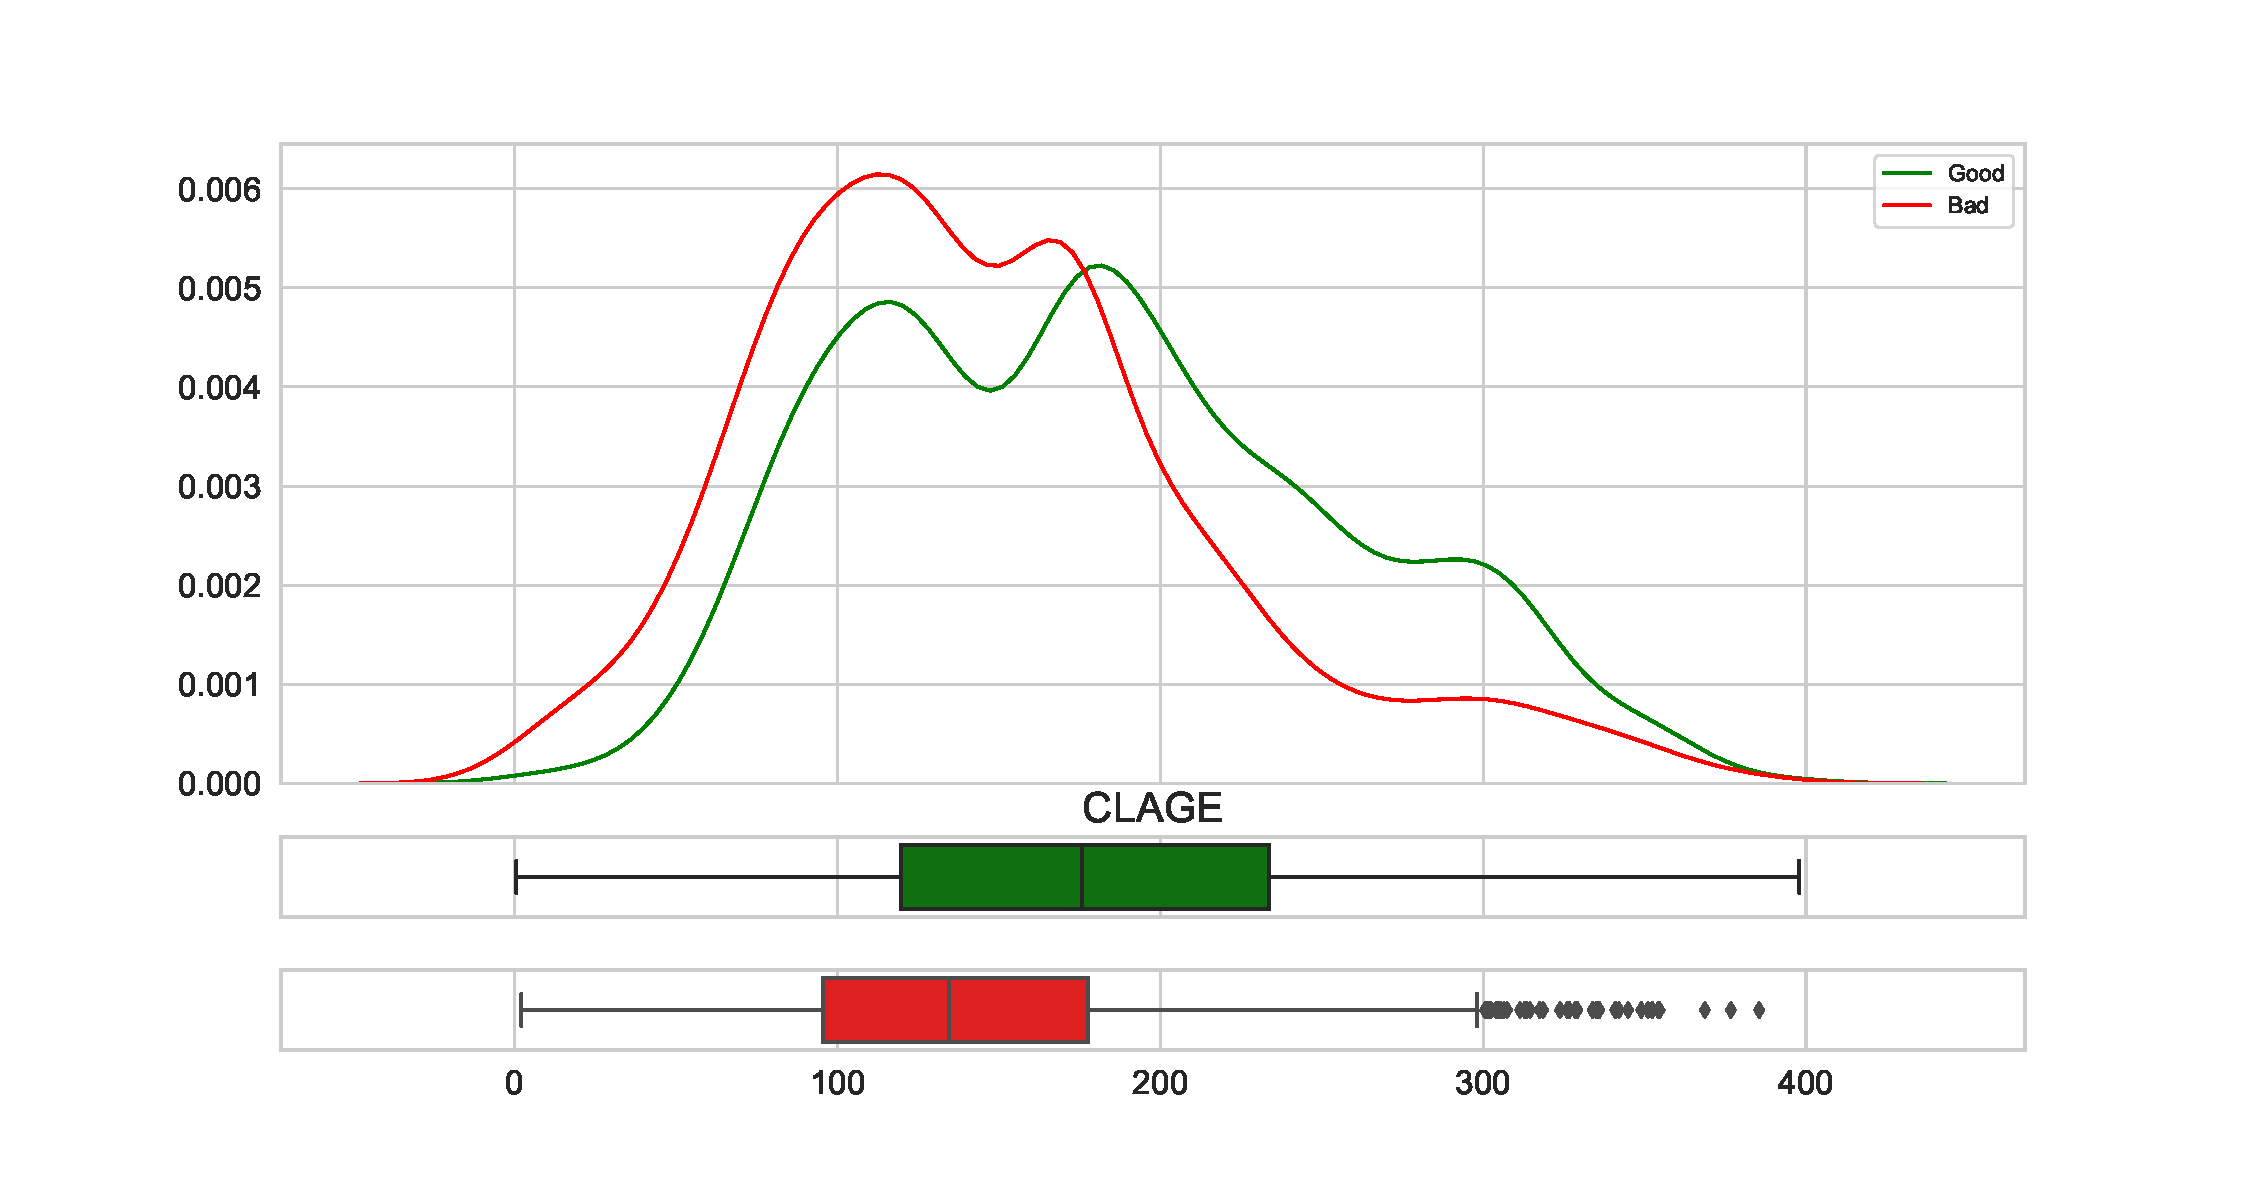
\includegraphics[scale=0.40]{figs/clage_dist.pdf}
	\caption{Distribution of CLAGE by BAD. \label{clage_dist}}
\end{figure}

\subsection*{NINQ}

NINQ,  number of recent credit inquiries. Figure (\ref{ninq_cat}) indicates that the more recent credit equiries an applicant makes the more likely they are to default,  this trend is followed until the higher values are reached but this deviation could be due to the low sample size at larger values. 73.8\% of applicants have made no more than 1 recent credit equiry where as only 3\% of applicants made 5 or more. This could create an issue depending on how the WOE method bins the values.

\begin{figure}[H]
	\centering
	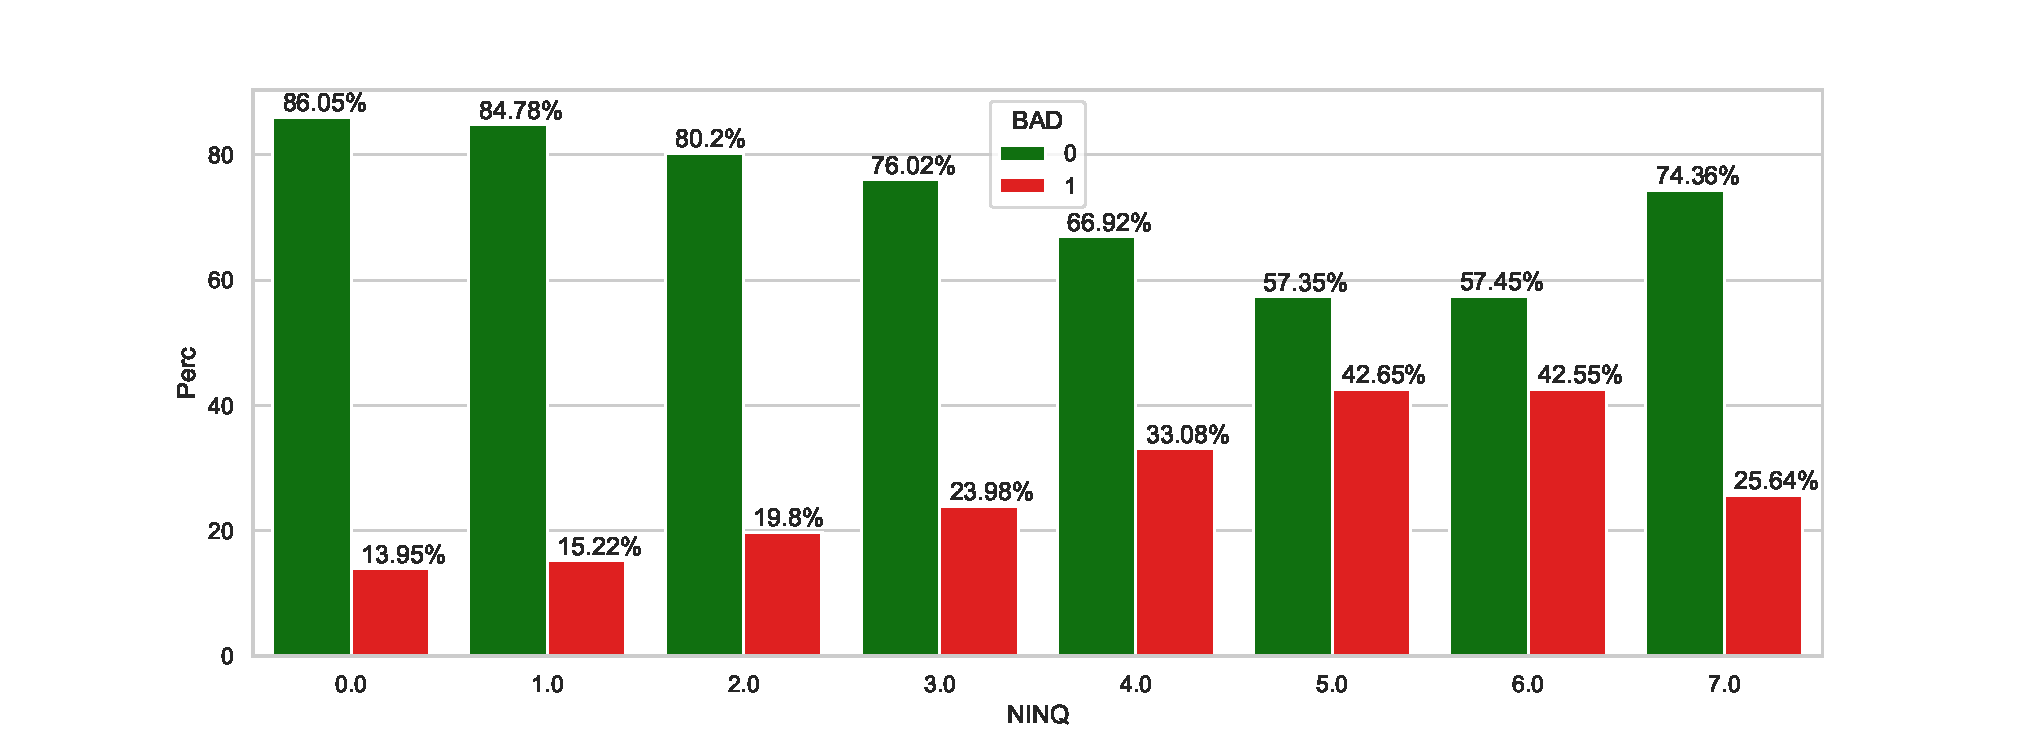
\includegraphics[scale=0.40]{figs/ninq_cat.pdf}
	\caption{Category plot of NINQ by BAD. \label{ninq_cat}}
\end{figure}

\subsection*{CLNO}

CLNO,  number of credit lines. A credit line can be any method in which someone can recieve credit such as an overdraft,  credit card,  etc. Figure (\ref{clno_dist}) suggests that applicants with low or high values for credit lines have a higher bad rate that ones in the centre. A reason behind this could be that a applicant with a low number of credit lines could be inexperience with debt management or don't have access to other credit to ensure payment on loans is on time. On the other end it could be that applicants with a large number of credit lines become incapable of managing the potential debt from the numerous sources. Where as the centre is seen to be where applicants have a good control over their credit lines. Applicants with a CLNO value between 20 and 30 have a bad rate of 15.1\% where applicants outside of this group have a bad rate of 23.1\%. A differnce of 8\%.

\begin{figure}[H]
	\centering
	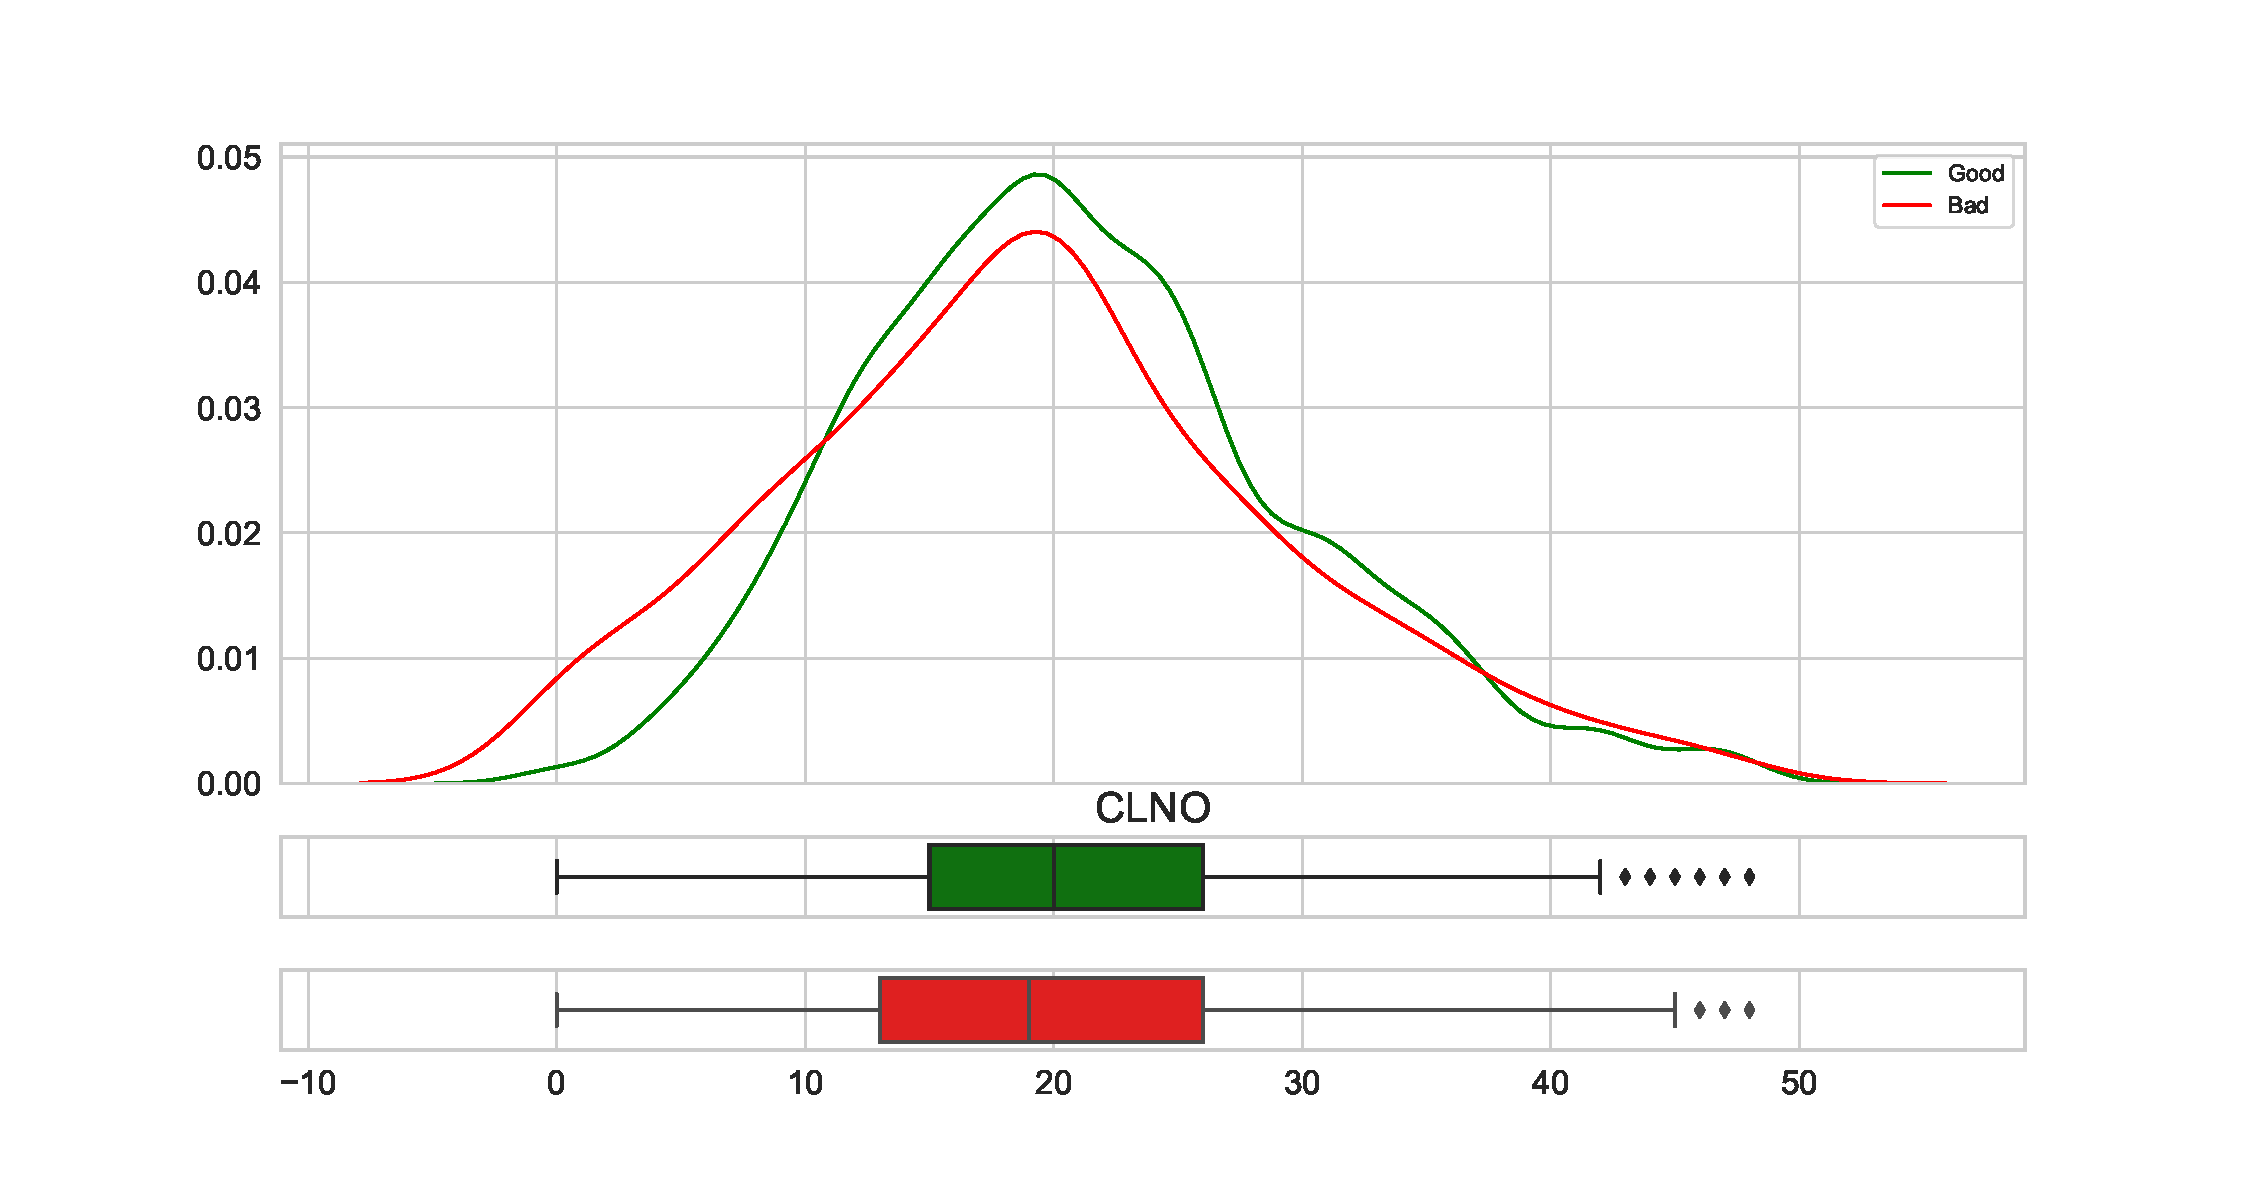
\includegraphics[scale=0.40]{figs/clno_dist.pdf}
	\caption{Distribution of CLNO by BAD. \label{clno_dist}}
\end{figure}

\section{WOE and IV}

WOE binning and calculation was done using the scorecardpy package provided by ShichenXie \parencite{scorecardpy},  results can be found in the two Tables (\ref{woe_1}) \& (\ref{woe_2}). I allowed the function to determine optimal bins itself using the chimerge method described in Section \ref{chimerge}. In the table we have a breakdown for each bin providing their woe value and individual information values. We can also see the total information value of each variable in the last column (total\_iv). Based on IV,  our strongest predictor by a large margin is DELINQ with a IV value of 0.40 and our weakest is Reason with an IV of 0.02. Referring back to Bailey's guideline (\ref{IV})\parencite{bailey2004credit}, we can categorise each variable on their strength from the IV.\\

Looking back on our data exploration we can see that our assumption about some of the variables appear to be reflecting in the WOE bins. Reason, a variable I expected to be rather insignifcant due to the bad rate being similar in both categories has the lowest IV. NINQ appears to have been binned appropriately with the upper bin being [4.0, inf) meaning the drop in bad rate at 7.0, assumed to be from a small sample, should not have a siginicant effect on the woe value of the group. The assumption on CLAGE, the variable with the second highest IV, is also reflected in the WOE values with a clear trend appearing in the bad probabilities of each bin seen in Figure (\ref{fig:ClageWoe}). The increase in bad probability in bin [170.0, 180.0) is most likely an error created by the single imputation used in the data cleaning, referring to the summary table before cleaning, Table (\ref{SUM_BFR_TBL}), you can see the median is 173.63 which is within the bin not following the trend.

\begin{figure}[ht]\label{Table2}
	\centering
	\renewcommand{\arraystretch}{1.25}
	\begin{tabular}{llr}
	\multicolumn{3}{c}{Variables Prediction Strength}\\
	\hline
	Variable & \multicolumn{1}{c}{Strength} & IV\\ 
	\hline
	LOAN & Average & 0.28\\
	MORTDUE & Weak & 0.08\\
	VALUE & Average & 0.18\\
	REASON & Poor & 0.02\\
	JOB & Average & 0.11\\
	YOJ & Weak & 0.08\\
	DEROG & Average & 0.21\\
	DELINQ & Strong & 0.40\\
	CLAGE & Average & 0.29\\
	NINQ & Average & 0.10\\
	CLNO & Average & 0.15\\
	\bottomrule
	\end{tabular}
\end{figure}

\begin{figure}
\centering
  \centering
  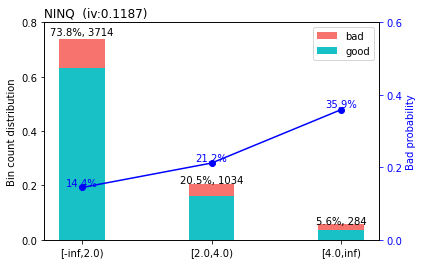
\includegraphics[width=0.9\linewidth]{figs/ninq_woe_plot.png}
  \caption{NINQ woe plot}
  \label{fig:NinqWoe}
\end{figure}

\begin{figure}
  \centering
 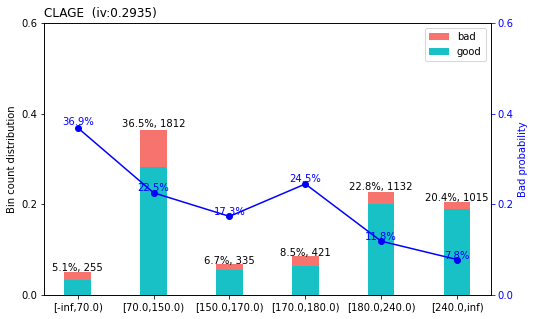
\includegraphics[width=0.9\linewidth]{figs/clage_woe_plot.png}
  \caption{Clage woe plot}
  \label{fig:ClageWoe}
\end{figure}

\begin{landscape}
	\begin{figure}[!ht]
		\centering
		\begin{tabular}{lllrrrrrrrr}
			\toprule
			variable & bin &  count &  count\_distr &  good &  bad &   badprob &       woe &    bin\_iv &  total\_iv \\
			\midrule
			    LOAN &      [-inf, 6000.0) &    250 &         0.05 &   125 &  125 &     0.50 &  1.54 &    0.17 &      0.28 \\
     &    [6000.0, 8000.0) &    276 &         0.06 &   202 &   74 &     0.27 &  0.54 &    0.02 &      0.28 \\
     &   [8000.0, 10000.0) &    428 &         0.09 &   352 &   76 &     0.18 &  0.01 &    0.00 &      0.28 \\
     &  [10000.0, 11000.0) &    259 &         0.05 &   199 &   60 &     0.23 &  0.34 &    0.01 &      0.28 \\
     &  [11000.0, 15000.0) &    927 &         0.19 &   778 &  149 &     0.16 & -0.11 &    0.00 &      0.28 \\
     &  [15000.0, 16000.0) &    296 &         0.06 &   226 &   70 &     0.24 &  0.37 &    0.01 &      0.28 \\
     &      [16000.0, inf) &   2534 &         0.51 &  2212 &  322 &     0.13 & -0.39 &    0.07 &      0.28 \\
			\midrule
			 MORTDUE &     [-inf, 35000.0) &    874 &         0.18 &   653 &  221 &     0.25 &  0.46 &    0.04 &      0.08 \\
  &  [35000.0, 55000.0) &   1139 &         0.23 &   928 &  211 &     0.19 &  0.06 &    0.00 &      0.08 \\
  &  [55000.0, 60000.0) &    341 &         0.07 &   293 &   48 &     0.14 & -0.27 &    0.00 &      0.08 \\
  &  [60000.0, 75000.0) &    854 &         0.17 &   697 &  157 &     0.18 &  0.05 &    0.00 &      0.08 \\
  &      [75000.0, inf) &   1762 &         0.35 &  1523 &  239 &     0.14 & -0.31 &    0.03 &      0.08 \\
			\midrule
			   VALUE &       [-inf, 50000.0) &    521 &         0.10 &   347 &  174 &     0.33 &  0.85 &    0.10 &      0.18 \\
    &    [50000.0, 70000.0) &    982 &         0.20 &   815 &  167 &     0.17 & -0.04 &    0.00 &      0.18 \\
    &    [70000.0, 80000.0) &    508 &         0.10 &   401 &  107 &     0.21 &  0.22 &    0.01 &      0.18 \\
    &   [80000.0, 125000.0) &   1922 &         0.39 &  1657 &  265 &     0.14 & -0.29 &    0.03 &      0.18 \\
    &  [125000.0, 175000.0) &    608 &         0.12 &   484 &  124 &     0.20 &  0.18 &    0.00 &      0.18 \\
    &       [175000.0, inf) &    429 &         0.09 &   390 &   39 &     0.09 & -0.76 &    0.04 &      0.18 \\
			\midrule
			  REASON &  DebtCon &   3442 &         0.69 &  2883 &  559 &     0.16 & -0.1 &    0.01 &      0.02 \\
   &  HomeImp &   1528 &         0.31 &  1211 &  317 &     0.21 &  0.2 &    0.01 &      0.02 \\
			\midrule
			      JOB &    Other &   2110 &         0.42 &  1666 &  444 &     0.21 &  0.22 &    0.02 &      0.11 \\
      &   Office &    844 &         0.17 &   746 &   98 &     0.12 & -0.49 &    0.03 &      0.11 \\
      &    Sales &     92 &         0.02 &    63 &   29 &     0.32 &  0.77 &    0.01 &      0.11 \\
      &  ProfExe &   1119 &         0.23 &   977 &  142 &     0.13 & -0.39 &    0.03 &      0.11 \\
      &      Mgr &    660 &         0.13 &   532 &  128 &     0.19 &  0.12 &    0.00 &      0.11 \\
      &     Self &    145 &         0.03 &   110 &   35 &     0.24 &  0.40 &    0.01 &      0.11 \\
			
			\bottomrule
		\end{tabular}
		\caption{WOE results table. \label{woe_1}}
	\end{figure}
	
	\begin{figure}[!ht]
		\centering
		\begin{tabular}{lllrrrrrrrr}
			\toprule
			variable & bin &  count &  count\_distr &  good &  bad &   badprob &       woe &    bin\_iv &  total\_iv \\
			\midrule
			      YOJ &   [-inf, 2.0) &    751 &         0.15 &   616 &  135 &     0.18 &  0.02 &    0.00 &      0.08 \\
      &    [2.0, 6.0) &   1139 &         0.23 &   880 &  259 &     0.23 &  0.32 &    0.03 &      0.08 \\
      &   [6.0, 10.0) &   1356 &         0.27 &  1155 &  201 &     0.15 & -0.21 &    0.01 &      0.08 \\
      &  [10.0, 23.0) &   1421 &         0.29 &  1162 &  259 &     0.18 &  0.04 &    0.00 &      0.08 \\
      &   [23.0, inf) &    303 &         0.06 &   281 &   22 &     0.07 & -1.01 &    0.04 &      0.08 \\
			\midrule
			   DEROG &  [-inf, 1.0) &   4442 &         0.89 &  3774 &  668 &     0.15 & -0.19 &    0.03 &      0.21 \\
    &   [1.0, inf) &    528 &         0.11 &   320 &  208 &     0.39 &  1.11 &    0.18 &      0.21 \\
			\midrule
			  DELINQ &  [-inf, 1.0) &   4050 &         0.81 &  3524 &  526 &     0.13 & -0.36 &    0.09 &       0.4 \\
	   &   [1.0, 2.0) &    537 &         0.11 &   367 &  170 &     0.32 &  0.77 &    0.08 &       0.4 \\
	   &   [2.0, inf) &    383 &         0.08 &   203 &  180 &     0.47 &  1.42 &    0.22 &       0.4 \\
			\midrule
			   CLAGE &    [-inf, 70.0) &    255 &         0.05 &   161 &   94 &     0.37 &  1.00 &    0.07 &      0.29 \\
	    &   [70.0, 150.0) &   1812 &         0.36 &  1404 &  408 &     0.23 &  0.31 &    0.04 &      0.29 \\
	    &  [150.0, 170.0) &    335 &         0.07 &   277 &   58 &     0.17 & -0.02 &    0.00 &      0.29 \\
	    &  [170.0, 180.0) &    421 &         0.08 &   318 &  103 &     0.24 &  0.41 &    0.02 &      0.29 \\
	    &  [180.0, 240.0) &   1132 &         0.23 &   998 &  134 &     0.12 & -0.47 &    0.04 &      0.29 \\
	    &    [240.0, inf) &   1015 &         0.20 &   936 &   79 &     0.08 & -0.93 &    0.13 &      0.29 \\
			\midrule
			     NINQ &  [-inf, 1.0) &   2192 &         0.44 &  1881 &  311 &     0.14 & -0.26 &    0.03 &       0.1 \\
	     &   [1.0, 3.0) &   2172 &         0.44 &  1785 &  387 &     0.18 &  0.01 &    0.00 &       0.1 \\
	     &   [3.0, 4.0) &    334 &         0.07 &   253 &   81 &     0.24 &  0.40 &    0.01 &       0.1 \\
	     &   [4.0, inf) &    272 &         0.05 &   175 &   97 &     0.36 &  0.95 &    0.06 &       0.1 \\
			\midrule
			     CLNO &  [-inf, 10.0) &    479 &         0.10 &   323 &  156 &     0.33 &  0.81 &    0.08 &      0.15 \\
     &  [10.0, 20.0) &   1882 &         0.38 &  1589 &  293 &     0.16 & -0.15 &    0.01 &      0.15 \\
     &  [20.0, 21.0) &    297 &         0.06 &   221 &   76 &     0.26 &  0.47 &    0.02 &      0.15 \\
     &  [21.0, 24.0) &    600 &         0.12 &   505 &   95 &     0.16 & -0.13 &    0.00 &      0.15 \\
     &  [24.0, 26.0) &    403 &         0.08 &   369 &   34 &     0.08 & -0.84 &    0.04 &      0.15 \\
     &   [26.0, inf) &   1309 &         0.26 &  1087 &  222 &     0.17 & -0.05 &    0.00 &      0.15 \\
			\bottomrule
		\end{tabular}
		\caption{WOE results table. \label{woe_2}}
	\end{figure}
\end{landscape}